\chapter{Livello Rete}
Il \emph{livello Rete} si occupa di trasferire i \emph{segmenti} ricevuti dal
\emph{livello Trasporto} alla rete di destinazione indicata. Il mittente, in
particolare, dopo aver deciso la direzione in cui instradare i
\emph{pacchetti}, li incapsula all'interno di \emph{frame} del \emph{livello}
sottostante. Giunti a destinazione, i \emph{frame} e quindi i \emph{pacchetti}
vengono passati al \emph{livello} superiore per poi essere consegnati al
processo corretto.

Diversamente da quanto visto in precedenza, i protocolli del \emph{livello Rete}
non mettono in comunicazione diretta mittente e destinatario, bensì, ogni
\emph{router} trasmette i \emph{pacchetti} ad uno dei \emph{\gls{glos:router}}
ai quali è collegato, e quello ripete l'operazione fino a quando non si arriva
alla rete di destinazione.

\section{Funzioni del livello Rete}
Le funzionalità del \emph{livello Rete} possono essere ripartite in due categorie
in base alla loro scale: \emph{locale} o \emph{globale}.

Su scala \emph{locale} i \emph{router} eseguo l'operazione di \emph{inoltro},
o \emph{forwarding}, che consiste nello spostamento di un \emph{pacchetto} da
un'interfaccia del \emph{router} ad un'altra. Agisce invece su scala
\emph{globale} l'operazione di \emph{instradamento}, o \emph{routing}, che
permette di determinare il percorso di un \emph{pacchetto}. L'operazione di
\emph{instradamento} è realizzata da particolari algoritmi di \emph{routing}.

\bigskip\noindent
\emph{Inoltro} e \emph{instradamento} appartengono a due
\emph{piani} differenti che sono rispettivamente il \emph{piano dati} e il
\emph{piano controllo}.

Il \emph{piano dati}, o \emph{data plane}, è una funzione locale di ogni
\emph{router} che determina come inoltrare un \emph{pacchetto} da una porta di
entrata a una porta di uscita dello stesso.

Il \emph{piano controllo}, o \emph{control plane}, invece, gestisce la
logica globale della rete e lo fa determinando come instradare un
\emph{pacchetto} in un percorso \emph{end-to-end}, cioè dall'\emph{host}
mittente all'\emph{host} destinatario.

\begin{figure}[ht]
    \centering
    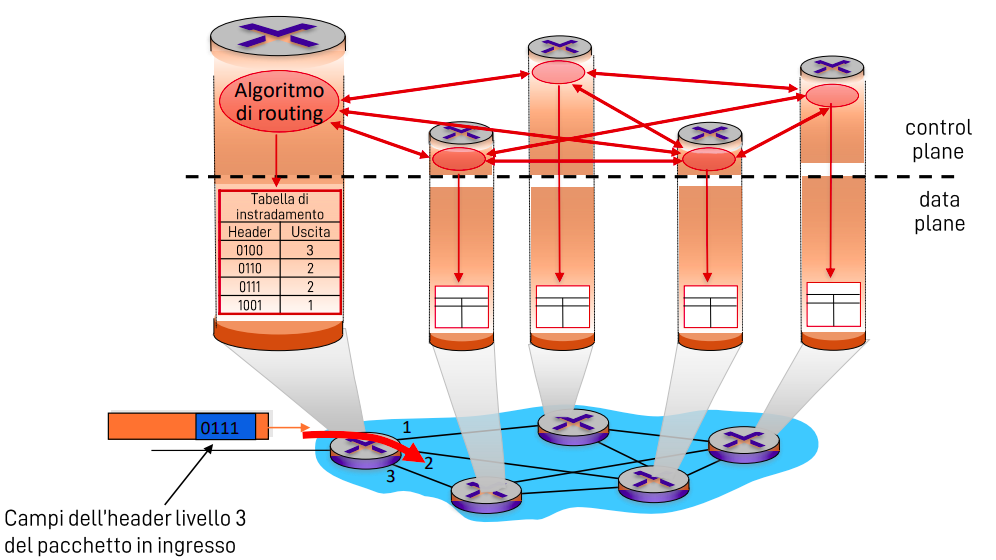
\includegraphics[width=\textwidth]{data-control-plane.png}
    \caption{\emph{Data plane} e \emph{control plane}}
\end{figure}
\newpage

\section{Struttura e funzionamento di un router}
\begin{figure}[h!]
    \centering
    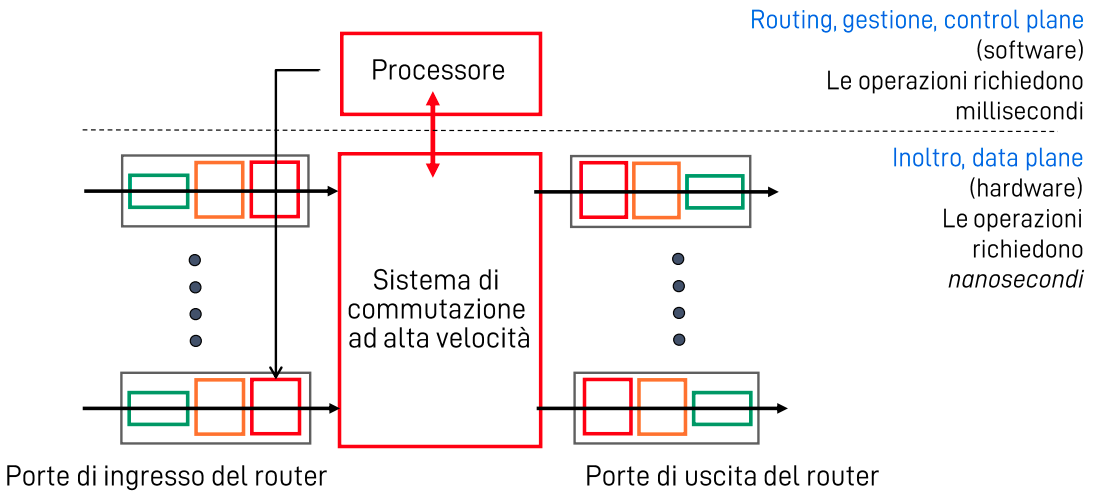
\includegraphics[width=\textwidth]{router.png}
    \caption{Struttura di un \emph{router}}
\end{figure}
\subsection{Porte di ingresso}
Ogni porta comprende tre componenti:
\begin{enumerate}
    \item \emph{Terminatore di linea}: riceve o invia i singoli bit;
    \item \emph{Livello Data Link}: un protocollo di \emph{livello Data Link}
    per l'interpretazione dei bit (e.g. \emph{Ethernet});
    \item \emph{Sistema di commutazione decentralizzato}: è un componente che
    utilizza i valori dell'\emph{header} di \emph{livello 3} per decidere,
    usando una tabella di inoltro salvata in ogni porta, verso quale porta in
    uscita inoltrare un \emph{pacchetto}.
\end{enumerate}
Il \emph{sistema di commutazione} di ogni porta è progettato in modo da
ridurre al minimo il tempo di elaborazione perché l'obiettivo è quello di non
introdurre ritardi eccessivi. In ogni caso, ogni porta è dotata di un buffer nel
quale vengono accodati i \emph{pacchetti} che devono essere \emph{inoltrati}.

\begin{figure}[h!]
    \centering
    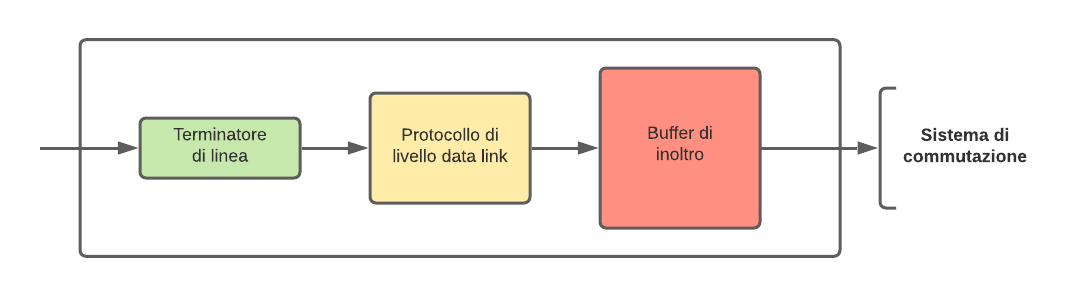
\includegraphics[width=\textwidth]{porta-ricezione.png}
    \caption{Porta di ingresso}
\end{figure}

\subsection{Sistemi di commutazione}
I sistemi di commutazione servono per trasferire i dati dalle porte di ingresso
a quelle di uscita. La frequenza alla quale i \emph{pacchetti} vengono trasferiti
dagli ingressi alle uscite è detta \emph{tasso di commutazione} e spesso è
misurato come multiplo della velocità di comunicazione, ovvero, con $N$ ingressi
avremo una commutazione $N$ volte più veloce della comunicazione.
Esistono tre tipi di sistemi di commutazione: a \emph{memoria}, a \emph{bus} e
a \emph{matrice}.

\paragraph{Commutazione a memoria}
Questo sistema veniva usato nelle prime generazioni di \emph{router} e di fatto
faceva funzionare i \emph{router} esattamente come i normali computer.
I \emph{pacchetti} venivano salvati in memoria, lì erano analizzati dalla CPU e
quindi inviati verso la porta d'uscita.

La velocità di commutazione era limitata dalla banda dati della memoria e, inoltre,
per ogni \emph{pacchetto} erano necessari due accessi al bus di sistema.

\begin{figure}[h]
    \centering
    \subfloat[\emph{Commutazione a memoria}]{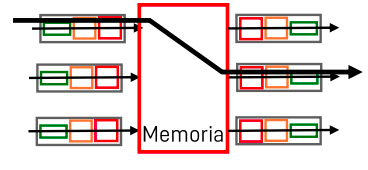
\includegraphics[width=0.33\textwidth]{comm-memoria.png}}
    \hfill
    \subfloat[\emph{Router} con \emph{commutazione a memoria}]{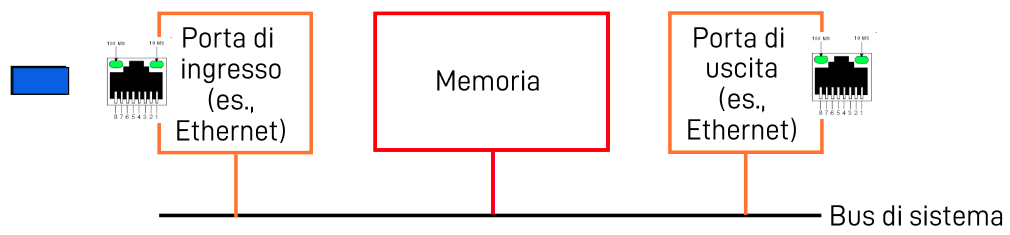
\includegraphics[width=0.63\textwidth]{comm-memoria-2.png}}
    \caption{\emph{Commutazione a memoria}}
\end{figure}

\paragraph{Commutazione a bus}
In questo sistema si usa un bus dati condiviso attraverso il quale vengono
trasferiti i \emph{pacchetti}. Ovviamente la velocità di commutazione è limitata
dalla banda del bus e i \emph{pacchetti} devono transitare uno per volta.

\begin{figure}[ht]
    \centering
    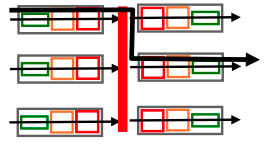
\includegraphics[width=0.33\textwidth]{comm-bus.png}
    \caption{\emph{Commutazione a bus}}
\end{figure}
\newpage

\paragraph{Commutazione a matrice}
Nei sistemi di commutazione a matrice vengono creati dei punti di
interconnessione tra le linee di ingresso e le linee di uscita. Questa
configurazione permette di superare i limiti di velocità della commutazione a
bus perché più \emph{pacchetti} possono transitare contemporaneamente.
Inoltre, i \emph{pacchetti} vengono frammentati in celle di lunghezza fissa.

\begin{figure}[h!]
    \centering
    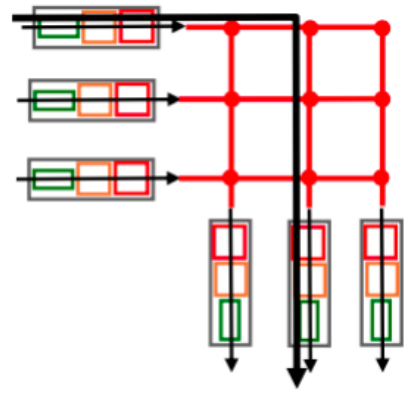
\includegraphics[width=0.33\textwidth]{comm-matrice.png}
    \caption{\emph{Commutazione a matrice}}
\end{figure}

\subsection{Conseguenze dei ritardi di commutazione}
Un commutatore più lento della velocità complessiva delle porte di ingresso
causa accodamenti agli ingressi e questo provoca ritardi e perdite nel caso
in cui i buffer si riempiano.

Si parla di \emph{Head of Line Block} (\emph{\gls{glos:HOL}}) quando un
\emph{pacchetto} che si trova in testa alla coda di un buffer impedisce a quelli
dietro di essere inoltrati. Questo blocco si verifica quando il commutatore è
occupato da un altro \emph{pacchetto} o quando la porta di uscita verso la quale
il \emph{pacchetto} in coda deve essere inoltrato è occupata dalla gestione di
un altro \emph{pacchetto}.

\begin{figure}[h!]
    \centering
    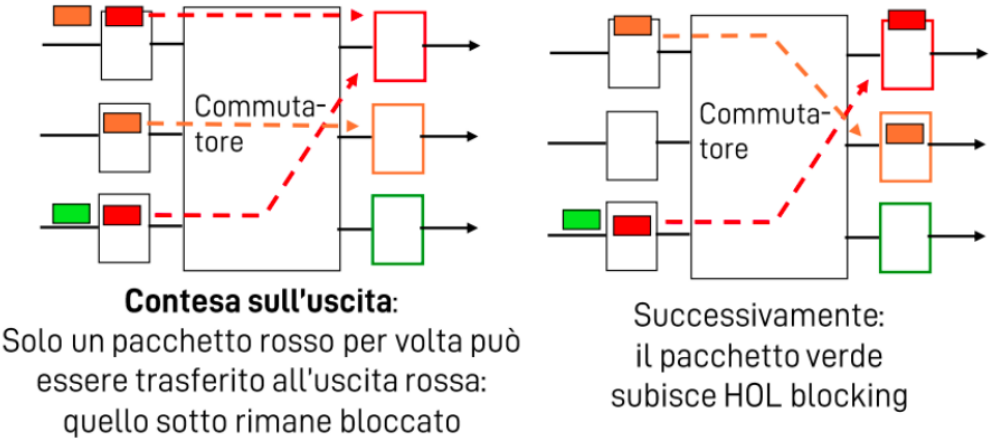
\includegraphics[width=0.7\textwidth]{head-of-line-block.png}
    \caption{\emph{Head of Line Block}}
\end{figure}

\subsection{Porte di uscita}
Le porte in uscita sono organizzate come quelle di ingresso, quindi con un
buffer, un protocollo di \emph{livello Data Link} e un terminatore di linea.
Il buffer serve a memorizzare i \emph{pacchetti} che devono essere spediti ed
esistono diverse politiche, dette \emph{polite di scheduling}, per la loro
gestione: \emph{FIFO} e \emph{Priority scheduling}.

La politica \emph{FIFO}, banalmente, invia i \emph{pacchetti} in base al loro
ordine di arrivo, mentre il \emph{priority scheduling} decide l'ordine di
invio sulla base della priorità assegnata ad ogni \emph{pacchetto}.

Qualora si opti per uno \emph{scheduling FIFO} bisogna comunque decidere come
gestire i pacchetti in eccesso che non possono essere memorizzati nel buffer.
Le cosiddette, \emph{politiche di scarto} sono tre:
\begin{itemize}
    \item \emph{Tail drop}: tutti i \emph{pacchetti} che non possono essere
    memorizzati vengono eliminati senza considerare altri parametri se non il
    tempo di arrivo;
    \item \emph{Priority drop}: vengono eliminati i \emph{pacchetti} con priorità
    più bassa in modo da fare spazio per gli altri;
    \item \emph{Random drop}: i \emph{pacchetti} da scartare vengono scelti
    casualmente;
\end{itemize}

\begin{note}
    Il \emph{priority scheduling} può andare in contrasto con quella che è la
    \emph{network neutrality}.
\end{note}

\begin{figure}[h!]
    \centering
    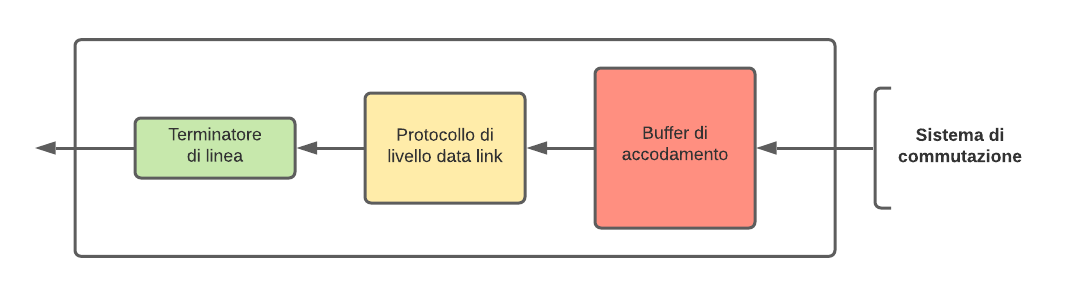
\includegraphics[width=\textwidth]{porta-invio.png}
    \caption{Porta di uscita}
\end{figure}

\paragraph{Dimensione dei buffer}
Raccomandazioni recenti affermano che con $N$ flussi di ingresso/uscita la
quantità di memoria richiesta da ogni buffer è espressa dalla seguente espressione:
\[BM=\frac{RTT\cdot R}{\sqrt{N}}\]

\section{Protocollo IP}
\subsection{Struttura dei pacchetti}
Un \emph{pacchetto \gls{prot:IP}} ha un header organizzato in parole da 32 bit.
I campi sono i seguenti:
\begin{itemize}
    \item \texttt{Versione} (4bit): numero di versione del protocollo \emph{IP} (4 o 6);
    \item \texttt{Lunghezza header} (4bit): numero di parole dell'header (5 se
    non ci sono opzioni);
    \item \texttt{Tipo di servizio} (8 bit): classe di servizio del \emph{pacchetto}.
    In pratica è poco usato, ma potenzialmente potrebbe essere sfruttato per usare
    funzioni dette \emph{DiffServ} e \emph{Explicit Congestion Notification};
    \item \texttt{Lunghezza totale} (16bit): numero totale di byte del
    \emph{pacchetto} includendo sia l'header che il payload;
    \item \texttt{Id del pacchetto} (16bit): numero, solitamente sequenziale,
    usato per identificare i frammenti di un \emph{pacchetto} e poterli poi
    riassemblare;
    \item \texttt{Flag} (3bit): i bit del campo specificano se si tratta del
    frammento di un \emph{pacchetto} più grande e in particolare se è l'ultimo;
    \item \texttt{Offset del frammento} (13bit): indica in quale punto del
    \emph{pacchetto} originale va inserito questo frammento (è espresso in
    multipli di 8byte);
    \item \texttt{\gls{glos:TTL}} (8bit): è un valore intero che viene impostato dal
    mittente. Ogni volta che il \emph{pacchetto} passa per un \emph{router} viene
    ridotto di 1 e quando arriva a zero viene eliminato;
    \item \texttt{Protocollo superiore} (8bit): specifica il protocollo di livello
    superiore usato dal payload;
    \item \texttt{Checksum dell'header} (16bit): è il complemento a 1 della somma
    di tutte le parole di 16bit dell'header;
    \item \texttt{Indirizzo IP sorgente} (32bit): indirizzo iniziale del mittente;
    \item \texttt{Indirizzo IP destinazione} (32bit): indirizzo della destinazione
    finale;
    \item \texttt{Opzioni IP}: solitamente è vuoto, ma può essere usato per
    controllare l'elaborazione e l'instradamento dei \emph{pacchetti};
    \item \texttt{Padding}: è un insieme di bit impostati a zero che vengono
    aggiunti se le opzioni non terminano ad un multiplo di 32bit per fare in
    modo che l'header sia un multiplo di 32bit;
\end{itemize}

\begin{figure}[h!]
    \centering
    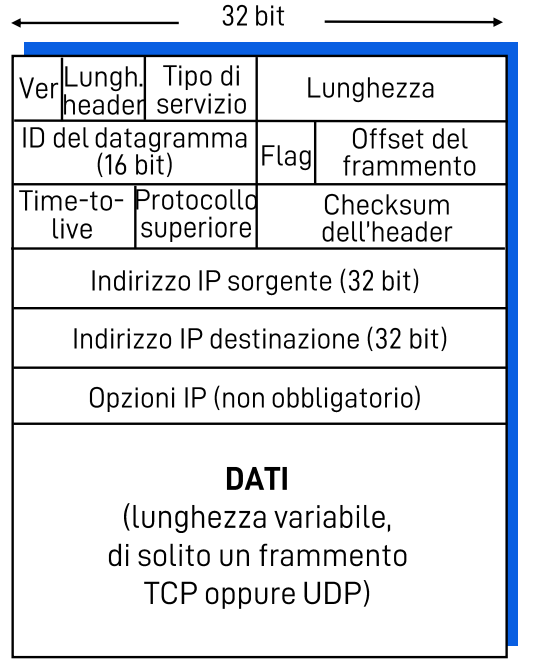
\includegraphics[width=0.47\textwidth]{pacchetto-ip.png}
    \caption{Struttura di un \emph{pacchetto IP}}
\end{figure}

\subsection{Frammentazione dei pacchetti}
Ogni \emph{pacchetto} ha una dimensione massima che corrisponde a un limite
imposto dall'hardware sul quale sta transitando. Questo valore limite è il già
citato in precedenza \emph{\gls{glos:MTU}}.

Poiché reti diverse possono avere \emph{MTU} diversi, può capitare che un
\emph{pacchetto} risulti troppo grande per essere inviato attraverso una di quelle
reti. Per questo motivo è possibile frammentare i \emph{pacchetti} in oggetti di
dimensione minore.

Il numero di frammenti necessari viene stabilito in base al valore di \emph{MTU}
e alla dimensione dell'header. Il payload viene quindi ripartito tra i frammenti
e in ciascuno di essi viene incluso lo stesso header del \emph{pacchetto}
originale. Ovviamente alcuni campi dell'header vengono modificati per includere
le informazioni necessarie alla gestione dei frammenti. In particolare viene
impostato il campo \texttt{Flag} $[0, D, M]$:
\begin{itemize}
    \item $D$: è il flag \quotes{Do not fragment} che quando è impostato indica
    al ricevitore di non frammentare il \emph{pacchetto} ed eventualmente di
    scartarlo se non fosse possibile inoltrarlo su una rete;
    \item $M$ è il flag \quotes{More fragments} e vale 1 su ogni frammento ad
    eccezione dell'ultimo;
\end{itemize}
Quando un \emph{pacchetto} viene frammentato, non viene più riassemblato fino
a quando non arriva al destinatario finale. Questo permette ai singoli frammenti
di seguire percorsi diversi e soprattutto evita che ogni \emph{router} debba
ricomporre e in caso riframmentare di nuovo il \emph{pacchetto}.

\begin{note}
    I \emph{router} che trattano i frammenti singolarmente indipendentemente gli
    uni dagli altri sono detti essere \emph{stateless}.
\end{note}\noindent
Ovviamente, fino a quando il ricevitore non ha ricevuto tutti i frammenti non
lì può ricomporre, quindi, quando arriva il primo frammento, il ricevitore
imposta un timer, allo scadere del quale, se non sono arrivati tutti i frammenti,
scarta quelli che ha memorizzato e ignora quelli che, in caso, dovessero arrivare.

\bigskip\noindent
Nella pratica però la frammentazione \emph{IP} non si usa e infatti molti
router non la implementano nemmeno. I motivi di questa scelta sono principalmente
legati alla sicurezza:
\begin{itemize}
    \item \emph{Attacchi \quotes{overlapping fragments}}: sono attacchi che puntano
    ad \quotes{ingannare} i \emph{router stateless} per permettere un traffico
    illecito di dati. Questo problema è risolvibile usando \emph{router statefull}
    che però sono più costosi e difficili da realizzare;
    \item \emph{Attacchi DDoS}: sono attacchi che puntano a congestionare un
    \emph{host} evitando di proposito di inviare alcuni frammenti e impedendo,
    quindi, la ricomposizione;
    \item Errate implementazioni del codice di riassemblaggio possono provocare
    un crash del codice dei \emph{router} permettendo così l'esecuzione di
    comandi arbitrari.
\end{itemize}
Inoltre, molti firewall si basano sull'ispezione degli header dei
protocolli di \emph{livello 4}, cosa che è impossibile con la frammentazione.

\subsection{Indirizzamento}
Gli \emph{indirizzi IP} sono stringhe di 32 bit che vengono associate ad
un'interfaccia di rete, che è un collegamento tra un \emph{host}, o un
\emph{router}, e un collegamento fisico. Ad ogni interfaccia possono essere
assegnati uno o più \emph{indirizzi} diversi, ma a interfacce diverse non possono
essere assegnati \emph{indirizzi} uguali. Gli \emph{indirizzi IP}
pubblicamente raggiungibili devono essere univoci in tutta la rete.

\paragraph{Struttura degli indirizzi IP}
Gli \emph{indirizzi IP} sono rappresentati mediante \quotes{dotted decimal notation},
ovvero, ogni byte codifica un valore intero positivo e ogni valore è separato
dagli altri con un punto. Poiché un byte è composto da 8 bit, il valore di ogni
ottetto va da $0$ a $255$ e quindi il range di \emph{indirizzi} va da
$0.0.0.0$ a $255.255.255.255$.

Generalmente, ogni \emph{indirizzo IP} è diviso in due parti:
\begin{itemize}
    \item \emph{NetID}: è la parte iniziale dell'\emph{indirizzo} e identifica
    la rete di appartenenza dell'\emph{host} al quale è stato assegnato. Ogni rete
    internet è identificata in modo univoco;
    \item \emph{HostID}: è la parte finale dell'\emph{indirizzo} e identifica
    una specifica interfaccia collegata ad una rete.
\end{itemize}
In particolare, tutti gli \emph{host} di una rete condividono lo stesso
\emph{NetID}, ma hanno \emph{HostID} diversi.

\begin{note}
    Nell'assegnamento degli \emph{indirizzi IP} bisogna garantire che ad ogni
    \emph{host} sia assegnato un \emph{indirizzo} univoco, che i \emph{NetID}
    siano coordinati a livello globale e che gli \emph{HostID} possano essere
    decisi localmente senza bisogno di un coordinamento globale.
\end{note}\noindent
Per garantire l'univocità dei prefissi di rete a livello globale, sono
stati istituiti degli enti appositi. Uno di essi è l'\gls{glos:ICANN}, un ente
che si occupa gestire l'assegnamento degli \emph{indirizzi} e la risoluzione di
controversie tra molteplici \quotes{pretendenti}. In realtà l'ICANN non distribuisce
direttamente gli \emph{indirizzi}, ma autorizza entità chiamate \emph{registrar}
a farlo. I \emph{registrar} permettono agli \emph{\gls{glos:ISP}} di
prendere in carico una parte degli \emph{indirizzi} e di distribuirli tra i
propri clienti.

\paragraph{Indirizzamento classful}
Ovviamente è necessario stabilire un modo per distinguere il \emph{NetID}
dall'\emph{HostID}. Inizialmente si era pensato ad un meccanismo a classi nel
quale ogni classe stabiliva un numero fisso di bit da dedicare al \emph{NetID}.

\begin{figure}[h!]
    \centering
    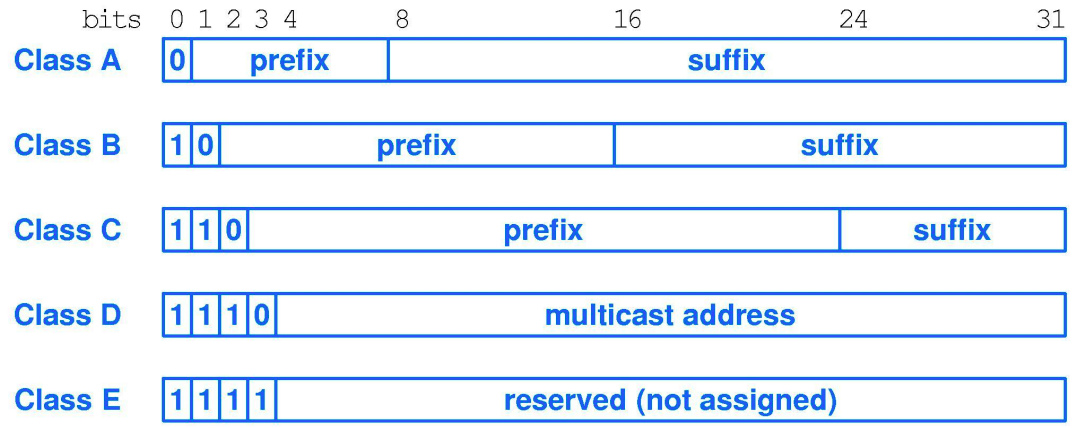
\includegraphics[width=\textwidth]{classi-ip.png}
    \caption{Classi di \emph{indirizzi IP}}
\end{figure}\noindent
Tuttavia, il sistema a classi si è rivelato inadatto in quanto gli utenti
preferivano utilizzare classi con una porzione più ampia di indirizzi
assegnabili, cosa che poi risultava in uno spreco.

\paragraph{Indirizzamento classless}
Con questo sistema, la suddivisione tra \emph{NetID} e \emph{HostID} è
arbitraria e può essere fatta sulla base delle necessità di un utente.

Per esempio, se un'azienda necessitasse di 57 \emph{indirizzi}, col sistema
classful sarebbe necessario un \emph{indirizzo} di classe C, che fornisce 256
\emph{indirizzi}\footnote{Vedremo più avanti che in realtà sarebbero 254},
quando in realtà un \emph{HostID} da 6 bit offrirebbe una suddivisione più
efficiente.

\noindent
Il sistema classless permette di assegnare un prefisso di 26 bit e un suffisso
da 6 ad un qualsiasi \emph{indirizzo}.  In pratica, se un \emph{ISP} avesse
a disposizione un indirizzo di classe C, potrebbe suddividere ulteriormente lo
spazio di indirizzi \quotes{allungando} il \emph{NetID}.

\begin{eg}[Suddivisione di un indirizzo di classe C]
Ad esempio, il seguente indirizzo di classe C:
\[193.185.15.0\]
corrisponde ad uno spazio di indirizzamento che va da
$11000001.10111001.00001111.00000000$ a
$11000001.10111001.00001111.11111111$.

Per suddividere lo spazio, l'ISP genera 4 NetID più lunghi:
\begin{itemize}
    \item \emph{NetID 1}: $11000001.10111001.00001111.00xxxxxx$;
    \item \emph{NetID 2}: $11000001.10111001.00001111.01xxxxxx$;
    \item \emph{NetID 3}: $11000001.10111001.00001111.10xxxxxx$;
    \item \emph{NetID 4}: $11000001.10111001.00001111.11xxxxxx$;
\end{itemize}
Ognuna di queste reti può contenere 62 host perché gli HostID
con tutti i bit impostati a 0 e a 1 sono riservati.
\end{eg}\noindent
Rimane comunque necessario stabilire un modo per distinguere il prefisso
dal suffisso. La soluzione è l'utilizzo di una \emph{netmask}, o maschera di rete,
costituita come una stringa di 32 bit nella quale gli unici bit impostati a 1
sono quelli del prefisso. \emph{Netmask} così definite permettono di risalire
al \emph{NetID} semplicemente eseguendo un AND bit-a-bit tra l'\emph{indirizzo}
di un \emph{host} e la maschera.

\begin{eg}[Applicazione di una netmask]
    Ad esempio, si prenda il seguente prefisso di rete:
    \[10000000.00001010.00000000.00000000 = 128.10.0.0\]
    con questa maschera:
    \[11111111.11111111.00000000.00000000 = 255.255.0.0\]
    Dato questo indirizzo:
    \[10000000.00001010.00000010.00000011 = 128.10.2.3\]
    l'AND bit-a-bit tra la netmask e l'indirizzo restituisce i primi 16 bit
    dell'indirizzo, ovvero:
    \[10000000.00001010.00000000.00000000 = 128.10.0.0\]
    che corrisponde proprio al prefisso di rete.
\end{eg}\noindent
Se notiamo, una maschera non è altro che una stringa di bit nella quale i primi
tot bit sono impostati a 1 (e.g. nell'\hyperref[eg:2]{esempio 2} sono i primi 26).
Quindi, invece di indicare esplicitamente la maschera, è possibile usare la
notazione \emph{\gls{glos:CIDR}} e scrivere l'\emph{indirizzo} seguito da $/x$
dove $x$ è il numero di bit a 1 (e.g. nell'esempio 2 scriveremmo $/26$).

\begin{eg}[Appliazione della notazione CIDR]
    Si supponga che un ISP possieda il seguente blocco di indirizzi:
    \[128.211.0.0/16\]
    e che abbia tre clienti che necessitano rispettivamente di 12, 9 e 6
    indirizzi.

    Date le richieste, l'ISP calcola che ad ogni cliente serviranno 4, 4 e 3 bit
    per l'HostID, che corrispondono a 28, 28 e 29 bit di netmask.

    Quindi, i 3 clienti potrebbero ricevere i seguenti indirizzi:
    \begin{itemize}
        \item Cliente 1: $128.211.0.16/28$;
        \item Cliente 2: $128.211.0.32/28$;
        \item Cliente 3: $128.211.0.48/28$;
    \end{itemize}
\end{eg}
\begin{note}
    I primi due clienti hanno prefissi diversi, ma la stessa maschera.
\end{note}\noindent
Ovviamente, quando a un cliente vengono assegnati degli indirizzi, questo può
assegnarli ai propri \emph{host} come meglio crede.

\paragraph{Conversione binario-decimale delle netmask}
\mbox{}\\
\begin{minipage}[t]{0.48\textwidth}\vspace{-3mm}
    \begin{itemize}
        \item $10000000 = 128 \Rightarrow /25$;
        \item $11000000 = 192 \Rightarrow /26$;
        \item $11100000 = 224 \Rightarrow /27$;
        \item $11110000 = 240 \Rightarrow /28$;
    \end{itemize}
\end{minipage}
\hfill
\begin{minipage}[t]{0.48\textwidth}\vspace{-3mm}
    \begin{itemize}
        \item $11111000 = 248 \Rightarrow /29$;
        \item $11111100 = 252 \Rightarrow /30$;
        \item $11111110 = 254 \Rightarrow /31$;
        \item $11111111 = 255 \Rightarrow /32$;
    \end{itemize}
\end{minipage}\vspace{0.5mm}
Le maschere $/31$ e $/32$ non hanno senso di esistere perché non forniscono
\emph{indirizzi assegnabili}.

\paragraph{Regole di inoltro}
Quando un \emph{router} riceve un \emph{pacchetto}, per decidere su quale
interfaccia inoltrarlo, utilizza soltanto l'\emph{indirizzo IP} di destinazione.

In particolare, ogni \emph{router} gestisce una tabella di inoltro nella quale
ad ogni interfaccia vengono assegnati gli indirizzi che permette di raggiungere.

\begin{figure}[h!]
    \centering
    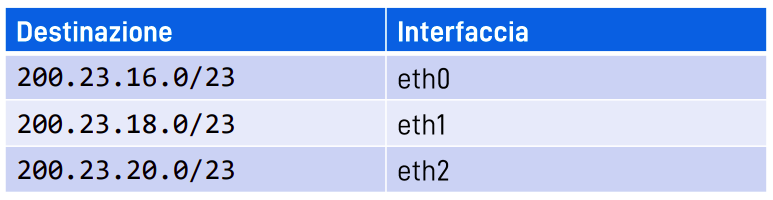
\includegraphics[width=0.7\textwidth]{tabella-inoltro-1.png}
    \caption{Esempio di tabella di inoltro}
\end{figure}\noindent
Dato un \emph{indirizzo} di destinazione, partendo dalla prima entry della
tabella, si esegue l'AND bitwise tra l'\emph{indirizzo} da inoltrare e la
\emph{netmask} indicata nelle singole entry. Viene individuata una corrispondenza
quando il risultato dell'AND corrisponde all'\emph{indirizzo} della entry.

\begin{eg}[Scelta dell'interfaccia di inoltro]
    Valga la tabella di inoltro di cui sopra e sia $200.23.19.7$ l'indirizzo da
    inoltrare.

    \noindent
    Il router inizia a calcolare l'AND bitwise tra l'indirizzo da inoltrare e le
    varie netmask:
    \[200.23.19.7\ \&\ 255.255.254.0\ (/23)\ \Rightarrow\ 200.23.18.0\]
    In questo caso, l'indirizzo di inoltro è quello associato all'interfaccia
    \texttt{eth1} e quindi il pacchetto viene trasmesso a quell'interfaccia.
\end{eg}

\begin{eg}[Corrispondenze multiple]
    Si consideri la seguente tabella di inoltro:
    \begin{figure}[h!]
        \centering
        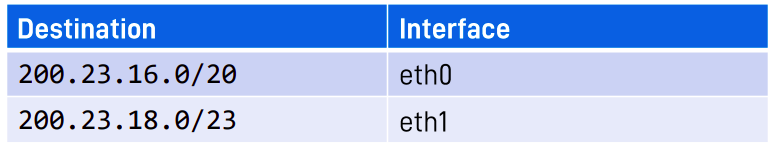
\includegraphics[width=0.7\textwidth]{tabella-inoltro-2.png}
    \end{figure}

    \noindent Dovendo inoltrare lo stesso indirizzo di prima:
    \[200.23.19.7\]
    si riscontra una corrispondenza con entrambe le entry, infatti:
    \[200.23.19.7\ \&\ 255.255.240.0\ (/20)\Rightarrow\ 200.23.16.0\]
    \[200.23.19.7\ \&\ 255.255.254.0\ (/23)\Rightarrow\ 200.23.18.0\]
    In questo caso si segue la regola del \quotes{longest prefix matching} e si
    sceglie come interfaccia di inoltro quella associata all'indirizzo con
    prefisso più lungo.
\end{eg}\noindent
Questo meccanismo di funzionamento delle tabelle di inoltro permette anche di
aggregare più percorsi in un'unica interfaccia e, contemporaneamente, di destinare
ad un'altra interfaccia i \emph{pacchetti} indirizzati verso un \emph{indirizzo}
più specifico.

\begin{figure}[h!]
    \centering
    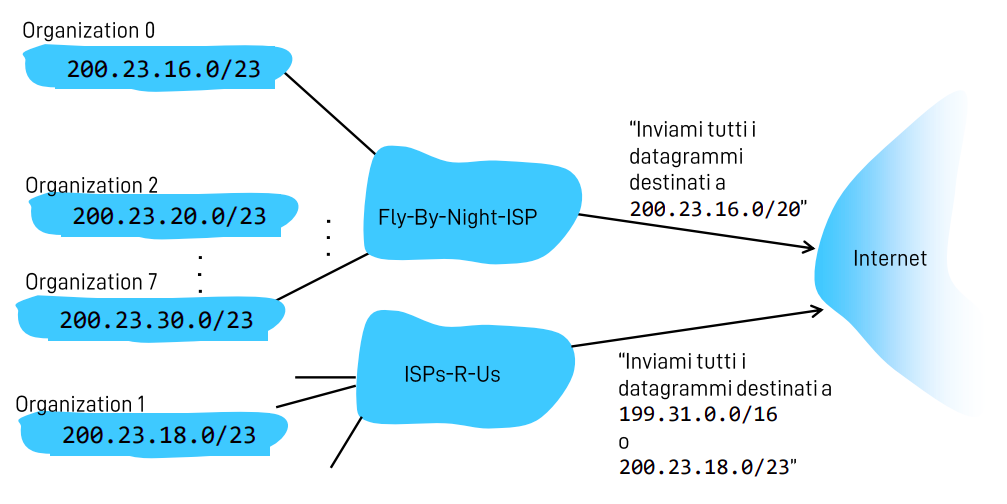
\includegraphics[width=0.9\textwidth]{aggregazione-indirizzi.png}
    \caption{Aggregazione di \emph{indirizzi} nelle tabelle di inoltro}
\end{figure}
\newpage
\begin{eg}[Aggregazioni e casi specifici]
    La tabella di inoltro associata all'immagine sopra è la seguente:
    \begin{figure}[h!]
        \centering
        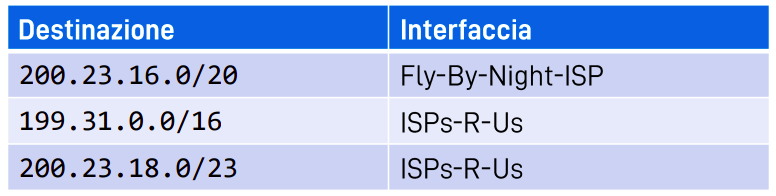
\includegraphics[width=0.7\textwidth]{tabella-inoltro-3.png}
    \end{figure}

    \noindent Dovendo inoltrare:
    \[200.23.19.7\]
    si rileva un riscontro con la prima e la terza entry, ma per la regola
    del \quotes{longest prefix matching} viene scelto $200.23.18.0/23$ e quindi
    l'interfaccia \texttt{ISPs-R-Us}.
\end{eg}\noindent
Nelle tabelle di inoltro esiste un'entry, l'ultima, che ha indirizzo $0.0.0.0/0$
e viene scelta quando nessuna nelle precedenti ha generato un riscontro.
Questo valore è detto \emph{\quotes{default gateway}} e negli \emph{host}
corrisponde solitamente all'\emph{indirizzo} del \emph{router}, mentre i
\emph{router} indicano l'\emph{indirizzo} di un altro \emph{router} che si
suppone sappia come inoltrare il \emph{pacchetto}.

\bigskip\noindent
L'ultimo caso da prendere in considerazione è quello in cui da un'interfaccia
siano raggiungibili più \emph{router}. In quel tipo di situazioni è necessario
sapere quale \emph{router} deve gestire la richiesta e per questo motivo, nelle
tabelle di inoltro, viene indicato, se serve, anche l'\emph{indirizzo IP} del
\emph{router} al quale inoltrare il \emph{pacchetto}. Quel valore viene
chiamato \emph{\quotes{next hop}}.

\begin{figure}[h!]
    \centering
    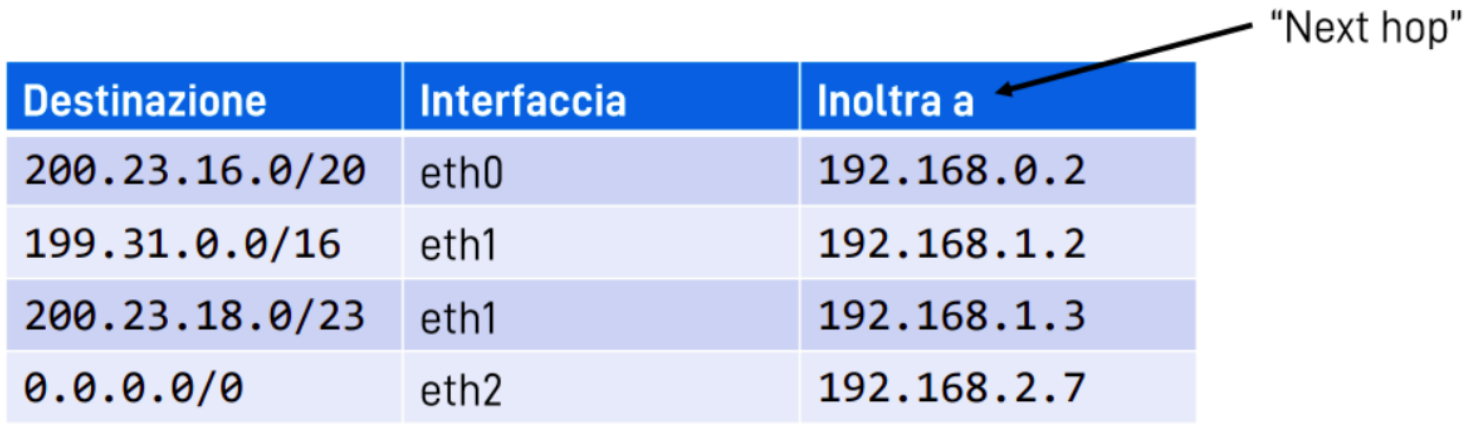
\includegraphics[width=\textwidth]{tabella-inoltro-4.png}
    \caption{Tabella di inoltro con \quotes{next hop}}
\end{figure}
\begin{note}
    Nonostante la presenza dell'\emph{indirizzo next hop}, gli \emph{indirizzi IP}
    di sorgente e di destinazione non cambiano!
\end{note}

\begin{eg}[Inoltro su reti contenenti più router]
    La seguente figura rappresenta lo schema di indirizzamento, con relativa
    tabella di inoltro, di una rete alla quale sono collegati più \emph{router}.
    \begin{figure}[ht]
        \centering
        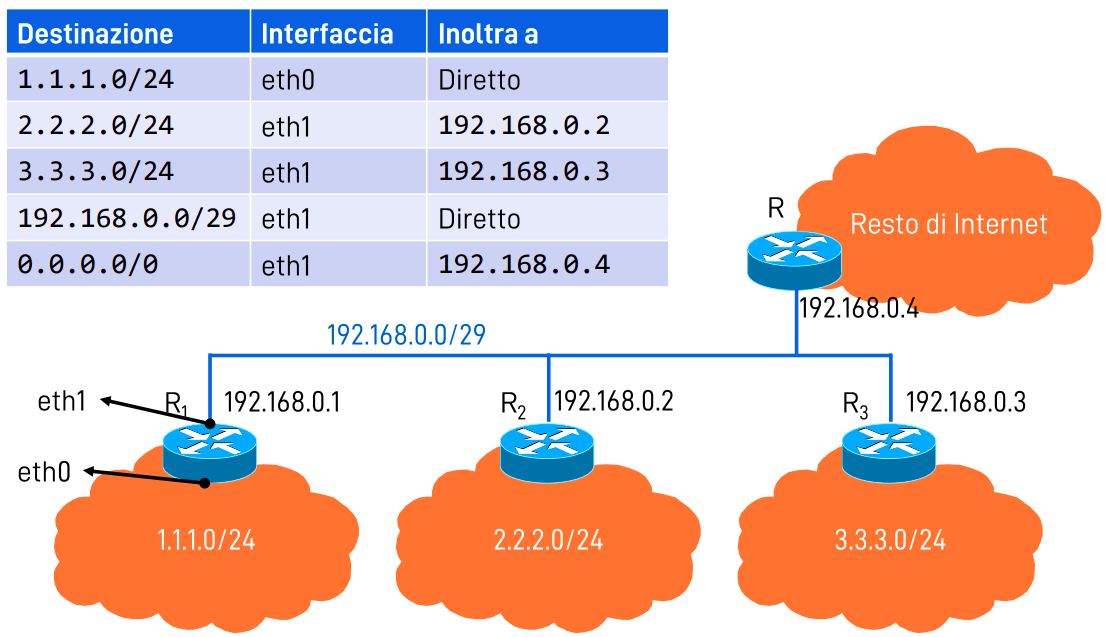
\includegraphics[width=0.85\textwidth]{reti-con-piu-router.png}
    \end{figure}
    \newpage
    \noindent In particolare, quando un pacchetto raggiunge il router
    $R1$, se è diretto verso la rete $1.1.1.0/24$, viene inoltrato verso
    l'interfaccia \texttt{eth0} senza indicare un indirizzo di \quotes{next hop}
    perché \texttt{eth0} è collegata direttamente alla rete da raggiungere.

    D'altra parte, l'interfaccia \texttt{eth1} è collegata alla rete $192.168.0.0/29$
    che è adiacente ad altre reti. Di conseguenza, i pacchetti destinati
    ad host che stanno nelle reti $2.2.2.0/24$ e $3.3.3.0/24$ dovranno
    essere inoltrati all'interfaccia \texttt{eth1}, passare attraverso la rete
    $192.168.0.0/29$ e raggiungere i router $R2$ e $R3$. Poiché $R2$ e $R3$
    sono raggiungibili agli indirizzi $192.168.0.2$ e $192.168.0.3$, quegli
    indirizzi sono stati indicati come indirizzi di \quotes{next hop}.

    Infine, i pacchetti destinati a reti non conosciute da $R1$ sono inviati al
    default gateway, che in questo caso, è il router $R$ all'indirizzo $192.168.0.4$.
\end{eg}

\begin{note}
    Tipicamente, le tabelle di routing presenti negli \emph{host} (non i
    \emph{router}), hanno una struttura simile alla seguente:
    \begin{figure}[h]
        \centering
        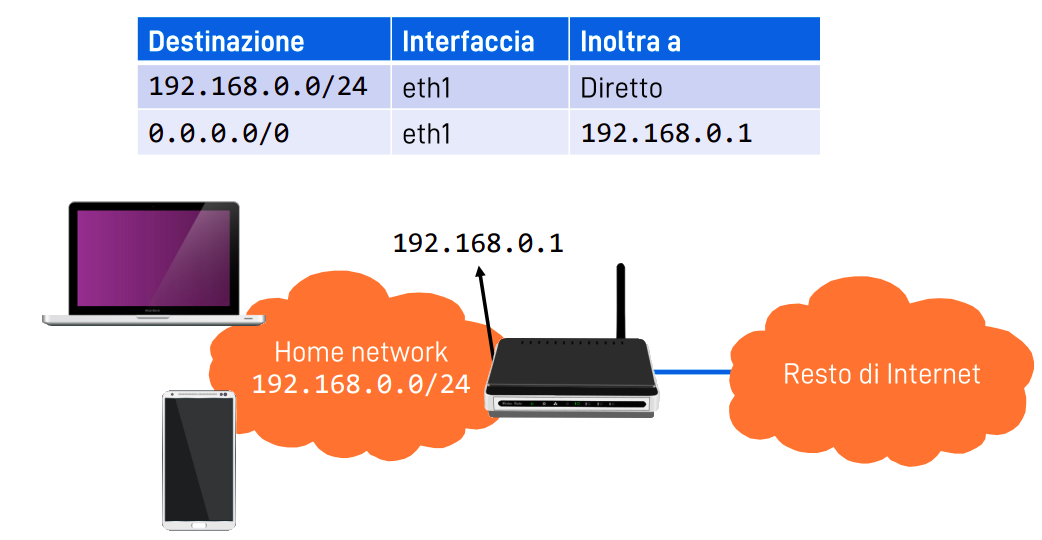
\includegraphics[width=0.85\textwidth]{tabella-routing-su-host.png}
        \caption{Generica tabella di routing di un \emph{host}}
    \end{figure}
\end{note}

\subsection{Indirizzi privati e NAT}
\paragraph{Indirizzi pubblici e privati}
Non tutti gli \emph{indirizzi IP} possibili sono \emph{pubblici}, ma ne esistono
alcuni che sono, per l'appunto, \emph{privati}. Questo tipo di indirizzi possono
essere usati soltanto all'interno di reti locali e non sono raggiungibili da
\emph{host} che risiedono in altre reti, infatti i \emph{router} sono quasi
sempre impostati per scartare i \emph{pacchetti} con indirizzi privati.
Ovviamente, all'interno di una rete locale, devono comunque essere univoci.

Gli indirizzi privati sono distribuiti in 3 blocchi:
\begin{itemize}
    \item $10.0.0.0/8$: da $10.0.0.0$ a $10.255.255.255$;
    \item $172.16.0.0/12$: da $172.16.0.0$ a $172.31.255.255$;
    \item $192.168.0.0/16$: da $192.168.0.0$ a $192.168.255.255$;
\end{itemize}

\paragraph{NAT}
Visto che non è possibile comunicare in rete con \emph{host} dotati di
\emph{indirizzi IP privati}, ci si potrebbe chiedere coma sia possibile per essi
inviare \emph{pacchetti}. Le soluzioni possibili sono due:
\begin{itemize}
    \item \emph{Proxy}: usare un computer dotato sia di un \emph{indirizzo
    pubblico} che di uno \emph{privato}. Questo computer riceve tutte le richieste
    verso l'esterno e le esegue per conto dei mittenti;
    \item \emph{\gls{glos:NAT}}: è un apparecchio che sostituisce l'\emph{IP} e
    il \emph{numero di porta} sorgenti di ogni \emph{pacchetto} con il proprio
    \emph{indirizzo IP}, che è pubblico, e un \emph{numero di porta} casuale
    generato al momento; 
\end{itemize}\noindent
In particolare, il \emph{NAT} gestisce una tabella di questo tipo:

\begin{figure}[h!]
    \centering
    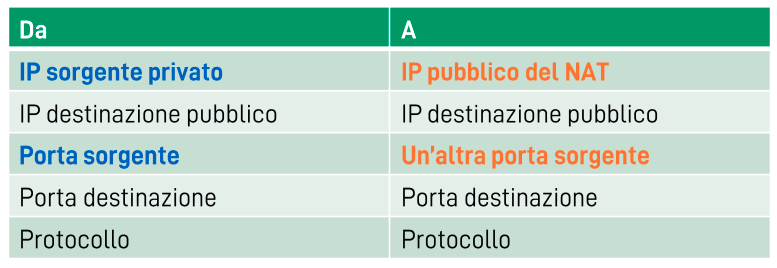
\includegraphics[width=0.8\textwidth]{tabella-nat.png}
    \caption{Tabella \emph{NAT}}
\end{figure}\noindent
Quando un \emph{host} della rete privata trasmette un \emph{pacchetto} che ha
per destinazione un \emph{indirizzo IP pubblico}, il \emph{NAT} inserisce in una
tabella una nuova entry, nella quale, l'\emph{indirizzo IP privato}
dell'\emph{host} e il \emph{numero di porta}, vengono associati all'\emph{indirizzo
pubblico} del \emph{NAT} e a un altro \emph{numero di porta} generato al momento.

Quindi, il \emph{pacchetto} viene ritrasmesso dal \emph{NAT} con le sorgenti
cambiate e quando l'\emph{host} destinatario risponde, il \emph{pacchetto} di
risposta viene nuovamente intercettato dal \emph{NAT} che sostituisce
l'\emph{indirizzo IP} e la \emph{porta} di destinazione con i valori salvati nella
tabella. A quel punto, il pacchetto può essere inoltrato alla sua destinazione.

\begin{figure}[ht]
    \centering
    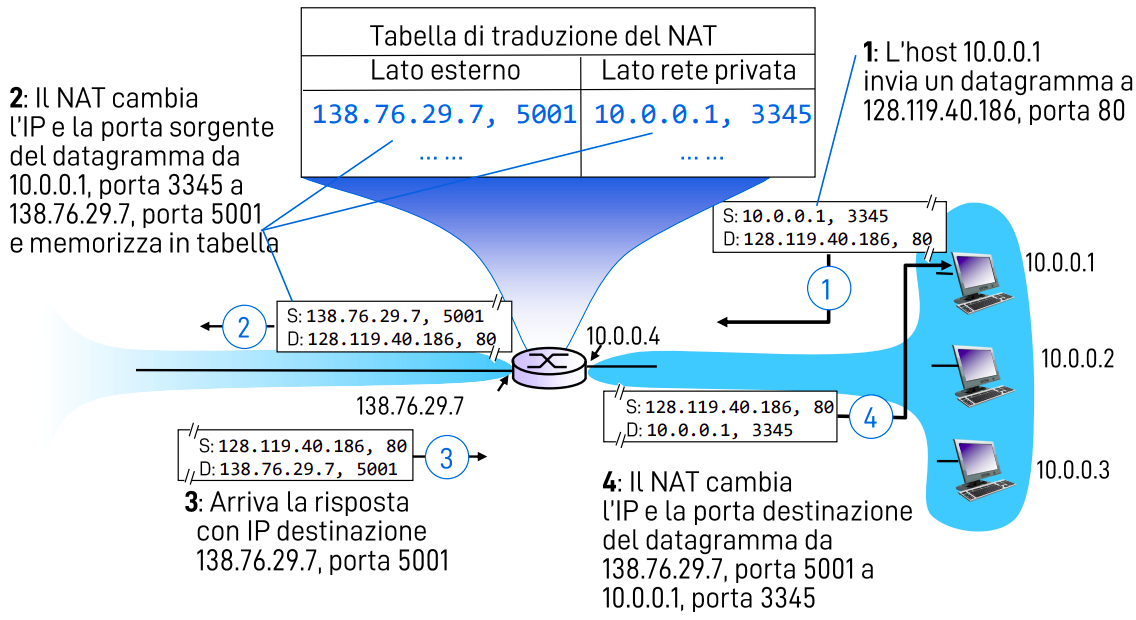
\includegraphics[width=0.9\textwidth]{esempio-nat.png}
    \caption{Esempio di utilizzo del \emph{NAT}}
\end{figure}
\newpage\noindent
Il \emph{NAT} è considerato una soluzione controversa in quanto porta con
se molti vantaggi, ma anche alcune problematiche.

Tra i vantaggi, si ha che il \emph{NAT} permette di ottenere fino a
$2^{16}\approx60000$ connessioni simultanee con un solo \emph{IP pubblico},
tamponando così il problema di carenza di indirizzi. Inoltre, il \emph{NAT}
impedisce a \emph{host} esterni alla rete di comunicare con gli \emph{host}
interni se non sono stati questi ad avviare la comunicazione, in quanto, se un
\emph{host} esterno tentasse di comunicare, il \emph{NAT} non saprebbe a chi
inoltrare i \emph{pacchetti} poiché non esisterebbe un'entry adatta nella tabella.

Quest'ultimo però è anche il primo degli svantaggi, perché i server devono poter
ricevere comunicazioni e quindi si vede necessario utilizzare degli espedienti
quali il \emph{port forwarding}, l'\emph{hole punching} o altri. Inoltre, il
\emph{NAT} viola due dei principi fondanti dell'architettura di internet: la
trasparenza e l'incapsulamento.

La trasparenza è violata perché il \emph{NAT} non è sempre trasparente ai
programmi applicativi e l'incapsulamento è violato perché vengono modificati gli
header di livello 3 e 4.

\begin{note}
    In certi casi il \emph{NAT} può essere l'unico modo di permettere a due
    \emph{host} di comunicare se non si controllano tutti i \emph{router} nel
    mezzo. Ad esempio, nella figura seguente l'\emph{host} a sinistra ha bisogno
    del \emph{NAT} sul \emph{router} $R$ per aprire una pagina sul server.

    \begin{figure}[h!]
        \centering
        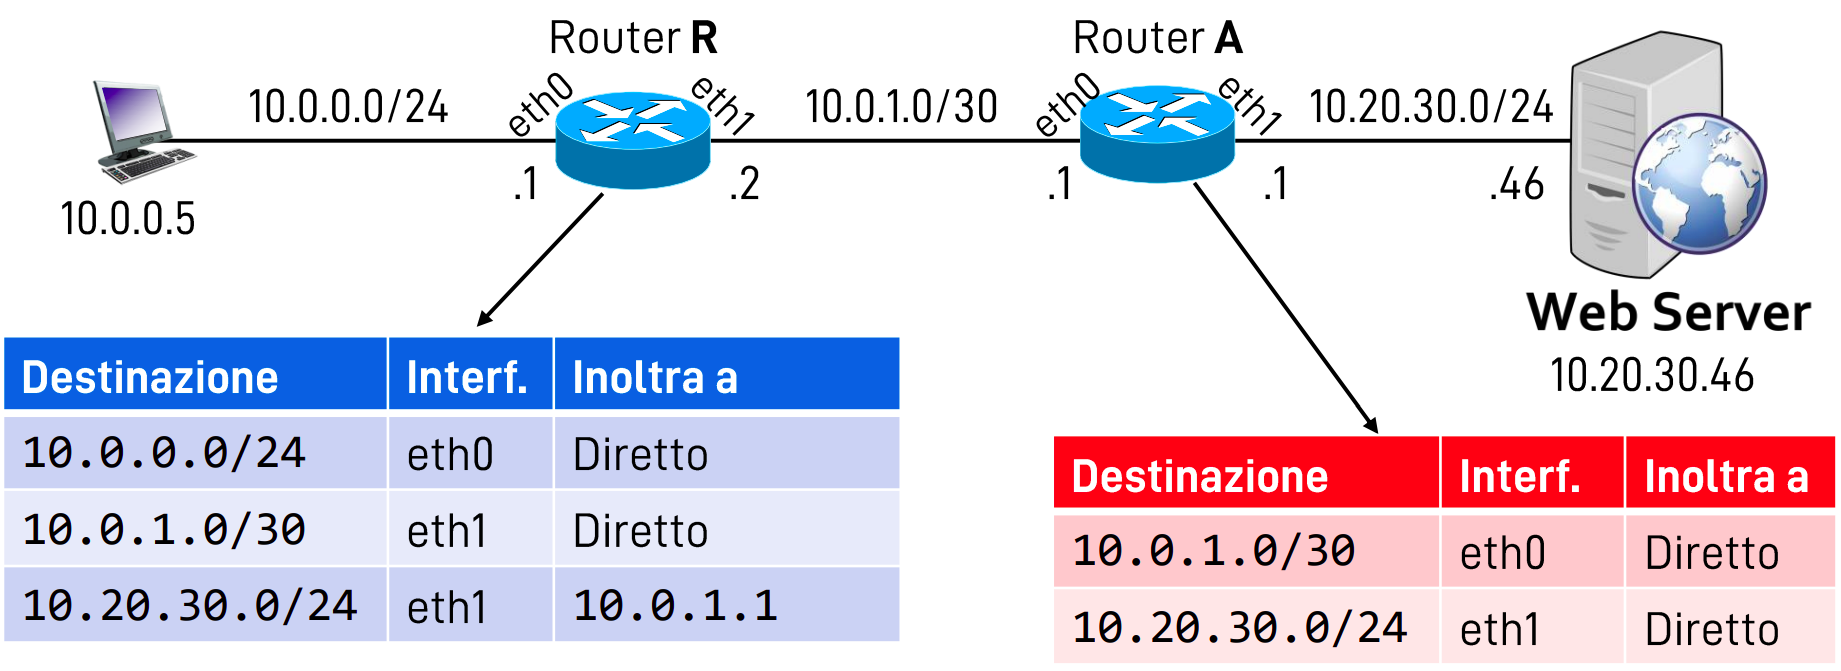
\includegraphics[width=0.9\textwidth]{esempio-vantaggio-nat.png}
        \caption{Esempio di necessità del \emph{NAT}}
    \end{figure}
\end{note}

\subsection{Indirizzi speciali}
Esistono alcuni \emph{indirizzi IP} che sono \quotes{speciali} e che hanno
significati particolari.

\paragraph{Indirizzi di rete}
Sono indirizzi usati per riferirsi al prefisso di una rete e son formati mettendo
a $0$ tutti i bit dell'\emph{HostID}.

Per esempio, $128.211.0.16/28$ è un \emph{indirizzo di rete} perché in binario
vale:
\[\underbrace{10000000.11010011.00000000.0001}_{\emph{NetID}}\underbrace{0000}_{\emph{HostID}}\]
D'altra parte, l'indirizzo $128.211.0.17/28$ non può essere un \emph{indirizzo di
rete} perché è codificato come:
\[\underbrace{10000000.11010011.00000000.0001}_{\emph{NetID}}\underbrace{0001}_{\emph{HostID}}\]
ma può essere un \emph{host} di quella rete.

\paragraph{Indirizzi di broadcast di rete}
Gli \emph{indirizzi di broadcast di rete} o \emph{directed broadcast addresses},
hanno tutti i bit dell'\emph{HostID} impostati a $1$ e si riferiscono a tutti
gli \emph{host} di una rete. I \emph{pacchetti} con questo tipo di indirizzi
vengono inoltrati dai \emph{router} in singola copia fino a quando non viene
raggiunto un \emph{router} della rete di destinazione, il quale, provvede a
consegnare una copia di quel \emph{pacchetto} ad ogni \emph{host} della rete.

Per esempio, data la rete $128.211.0.16/28$, l'\emph{indirizzo di broadcast di
rete} è:
\[\underbrace{10000000.11010011.00000000.0001}_{\emph{NetID}}\underbrace{1111}_{\emph{HostID}}\]

\paragraph{Indirizzo di broadcast di rete locale}
L'\emph{indirizzo di broadcast di rete locale} o \emph{limited broadcast
address} è un indirizzo in cui tutti i bit sono impostati a $1$ e si
riferisce a tutti gli \emph{host} di una rete, ovvero:
\[255.255.255.255\ \Rightarrow\ 11111111.11111111.11111111.11111111\]
La differenza con gli \emph{indirizzi di broadcast di rete} è che i \emph{pacchetti}
con questo indirizzo non vengono mai inoltrato dai \emph{router} e pertanto
rimangono confinati all'interno della rete locale.

\paragraph{Indirizzo \quotes{questo computer}}
Questo indirizzo è composto da 32 bit a $0$, ovvero:
\[0.0.0.0\ \Rightarrow\ 00000000.00000000.00000000.00000000\]
ed è usato dai computer quando sono stati appena avviati e non hanno ancora un
\emph{indirizzo IP}.

\paragraph{Indirizzi di loopback}
Gli \emph{indirizzi di loopback} sono tutti gli indirizzi appartenenti alla rete
$127.0.0.0/8$ e sono usati per testare applicazioni di rete in esecuzione su un
computer. In particolare, i pacchetti con questo indirizzo, discendono lo
\emph{stack protocollare} fino al livello 3 e quindi lo risalgono per essere
consegnati all'applicazione destinataria senza lasciare il computer.

\paragraph{Indirizzi multicast}
Gli \emph{indirizzi multicast} servono ad inviare \emph{pacchetti} ad un gruppo
di \emph{host} e sono indirizzi che iniziano con $1110$ e quindi sono compresi
tra $224.0.0.0$ e $239.255.255.255$.

La logica di funzionamento è uguale a quella degli \emph{indirizzi di broadcast
di rete} che consente di evitare di dover trasmettere più copie di uno stesso
\emph{pacchetto}. Il problema è che la maggior parte dei \emph{router} bloccano
i \emph{pacchetti} con \emph{indirizzi multicast} e quindi il loro utilizzo è
fortemente limitato.

\paragraph{Indirizzi link-local}
Gli \emph{indirizzi link-local} sono assegnati automaticamente agli \emph{host}
che non riescono a farsi assegnare un \emph{indirizzo IP}\footnotemark.

In particolare, gli \emph{host} scelgono casualmente uno degli indirizzi della
sottorete $169.254.0.0/16$ e possono quindi comunicare soltanto all'interno di
quella sottorete.

\footnotetext{Vedremo più avanti cosa significa}

\paragraph{Indirizzi IP per i router}
Ad ogni \emph{router} possono essere assegnai uno o più indirizzi, o meglio,
è possibile assegnare almeno un indirizzo ad ogni interfaccia.

\begin{figure}[h!]
    \centering
    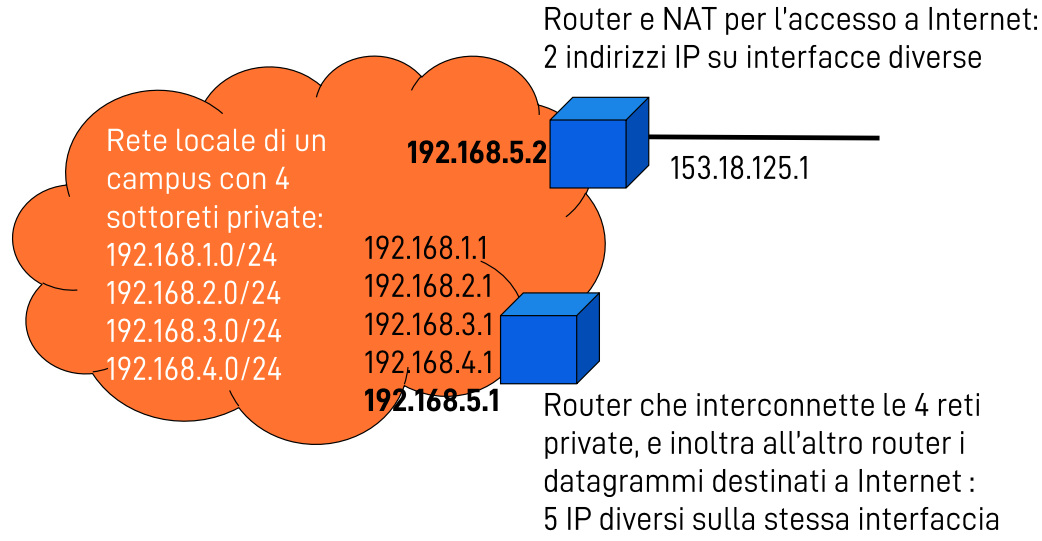
\includegraphics[width=0.8\textwidth]{router-con-piu-indirizzi.png}
    \caption{\emph{Router} con più indirizzi assegnati a un'interfaccia}
\end{figure}\noindent
Nella rete di questa immagine, tutto il traffico delle 4 sottoreti private viene
gestito dal \emph{router} in basso. Nel caso di traffico destinato all'esterno,
il \emph{router} trasmette quei \emph{pacchetti} al secondo \emph{router} e
questo poi li invia in rete. Questo sistema permette di dividere i \emph{domini
di broadcast}\footnotemark, ovvero limitare il numero di \emph{host} che ricevono
i \emph{pacchetti} con \emph{indirizzi di broadcast}, e alleggerire il carico
del secondo \emph{router}.

\footnotetext{Un \emph{dominio di broadcast} è l'insieme di tutti gli \emph{host}
che ricevono i \emph{pacchetti} trasmessi in \emph{broadcast}. C'è un'associazione
uno-a-uno tra \emph{sottorete} e \emph{dominio di broadcast}.}

\begin{note}
    Gli \emph{indirizzi di rete} e \emph{di broadcast di rete} sono il motivo per
    quale gli indirizzi assegnabili di una rete sono pari al numero di possibili
    \emph{host} rappresentabili meno 2.
\end{note}

\section{Protocollo ARP}
\subsection{Cenni sul livello 2}
Prima di passare alla trattazione del protocollo \emph{\gls{prot:ARP}} dobbiamo
chiarire alcuni dettagli sul livello 2.

Ogni \emph{pacchetto IP} viene incapsulato un \emph{frame} di livello 2 e per
poter trasmettere il \emph{frame} è necessario specificare gli indirizzi di
sorgente e di destinazione di quel livello. Questi indirizzi sono detti
\emph{indirizzi \gls{glos:MAC}} e sono stringhe di 48 bit, espresse come 12
cifre esadecimali, che identificano univocamente ciascuna interfaccia di rete.

\newpage
\subsection{Principi dell'ARP}
Dato che per trasmettere un \emph{frame} è necessario conoscere l'\emph{indirizzo
MAC} del destinatario deve esistere un protocollo che consenta di scoprirlo.
Il protocollo \emph{ARP} serve appunto a ricercare il \emph{MAC} associato ad
un'interfaccia con un certo \emph{indirizzo IP} noto a priori.

In particolare, l'\emph{host} che deve scoprire l'\emph{indirizzo MAC} trasmette
in broadcast una richiesta \emph{ARP} specificando l'\emph{IP} dell'interfaccia
dell'\emph{host} di cui ha bisogno di conoscere il \emph{MAC}. La richiesta
viene ricevuta da tutti gli \emph{host}, ma soltanto l'interessato risponde
specificando il proprio \emph{MAC}.

\begin{figure}[h!]
    \centering
    \subfloat[\emph{Richiesta ARP}]{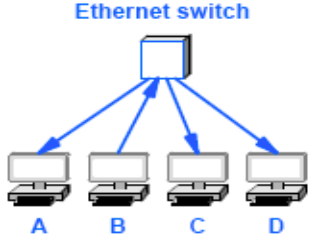
\includegraphics[width=0.48\textwidth]{richiesta-arp.png}}
    \hfill
    \subfloat[\emph{Risposta ARP}]{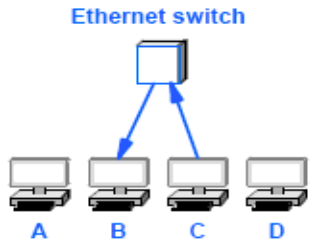
\includegraphics[width=0.48\textwidth]{risposta-arp.png}}
    \caption{Funzionamento del protocollo \emph{ARP}}
\end{figure}
\begin{note}
    Diversamente da quanto avviene a livello 3 in cui mittente e destinatario
    comunicano senza interessarsi degli \emph{host} nel mezzo, al livello 2
    tutte le comunicazioni sono punto-punto, quindi gli \emph{indirizzi MAC}
    cambiano ad ogni salto. Inoltre, quando si deve trasmettere un \emph{pacchetto}
    all'esterno della rete, non si cerca l'\emph{indirizzo MAC} dell'\emph{host}
    sull'altra rete, ma lo si lascia fare al \emph{router}.
\end{note}

\subsection{Messaggi ARP}
La seguente è la struttura di un messaggio \emph{ARP}:

\begin{figure}[h!]
    \centering
    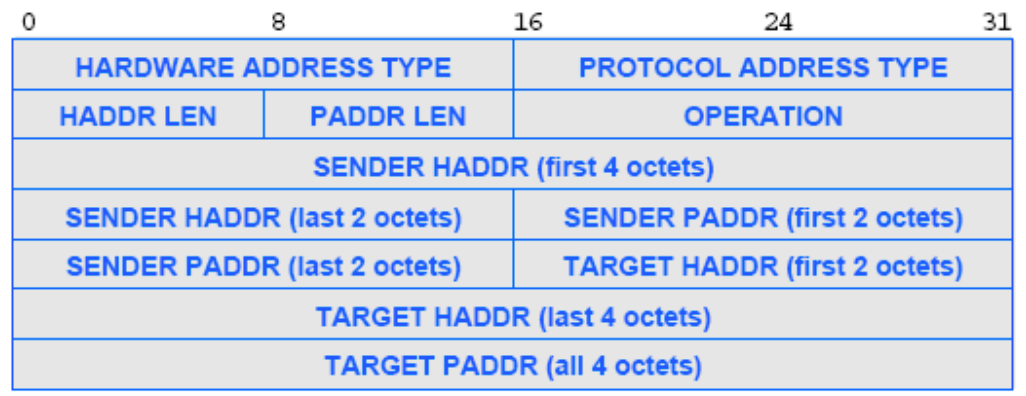
\includegraphics[width=0.7\textwidth]{messaggio-arp.png}
    \caption{Struttura di un messaggio \emph{ARP}}
\end{figure}\noindent
Con \texttt{Hardware Address} o \texttt{HADDR} ci si riferisce all'\emph{indirizzo
MAC}, mentre con \texttt{Protocol Address} o \texttt{PADDR} all'\emph{indirizzo
di livello 3}.
I messaggi \emph{ARP} vengono trattati come \emph{pacchetti} di livello 3 e quindi
sono incapsulati all'interno di \emph{frame} di livello 2.

\subsection{ARP caching}
Per evitare di dover trasmettere un messaggio \emph{ARP} per ogni \emph{pacchetto},
vengono mantenute in memoria le risposte \emph{ARP} ricevute in precedenza.

Le corrispondenze salvate vengono mantenute per 30 secondi prima di essere scartate
e nel caso in cui si ricevano nuove risposte \emph{ARP} relative a corrispondenze
già salvate, vengono sovrascritte le precedenti.

\subsection{Proxy ARP}
Nella situazione rappresentata nella figura seguente si ha un \emph{router} che
separa due gruppi di \emph{host} che quindi stanno su reti diverse.

\begin{figure}[h!]
    \centering
    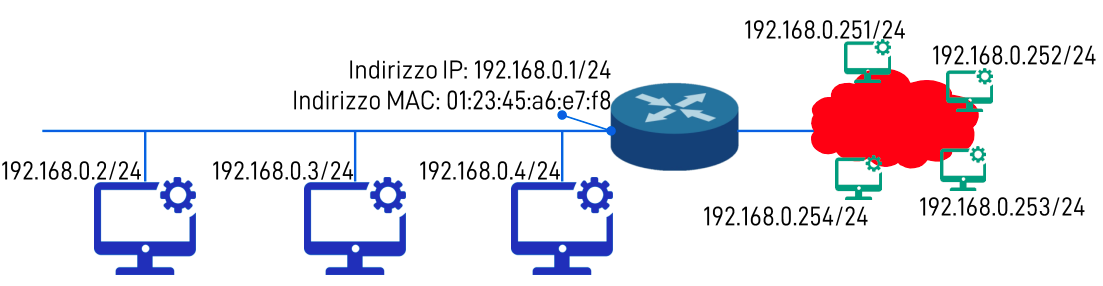
\includegraphics[width=\textwidth]{proxy-arp.png}
    \caption{\emph{Proxy ARP}}
\end{figure}\noindent
Tuttavia, possiamo notare che sia gli \emph{host} di sinistra che quelli
di destra hanno indirizzi della stessa sottorete $192.168.0.0/24$.

Questo è possibile perché il \emph{router} funge da \emph{proxy ARP}. Ovvero,
quando un \emph{host} sulla sinistra intende comunicare con un \emph{host}
sulla destra, o viceversa, invia una richiesta \emph{ARP} che viene intercettata
dal \emph{router} il quale risponde con il proprio \emph{indirizzo MAC}. A quel
punto, è il \emph{router} stesso che si incarica di inoltrare i \emph{pacchetti}
alla loro destinazione effettiva.

\section{Protocollo ICMP}
L'\emph{IP} include un protocollo ausiliario chiamato \emph{\gls{prot:ICMP}} che
viene usato per notificare errori all'\emph{host} mittente di un \emph{pacchetto}
e per trasportare altre informazioni utili.

\emph{IP} e \emph{ICMP} sono interdipendenti in quanto l'\emph{IP} usa \emph{ICMP}
per segnalare errori e i \emph{pacchetti ICMP} viaggiano su \emph{pacchetti IP}.

\subsection{Messaggi ICMP}
La struttura dei messaggi \emph{ICMP} è estremamente semplice. L'header si compone
soltanto di 3 campi: \texttt{type}, \texttt{code} e \texttt{checksum}.
\begin{figure}[ht]
    \centering
    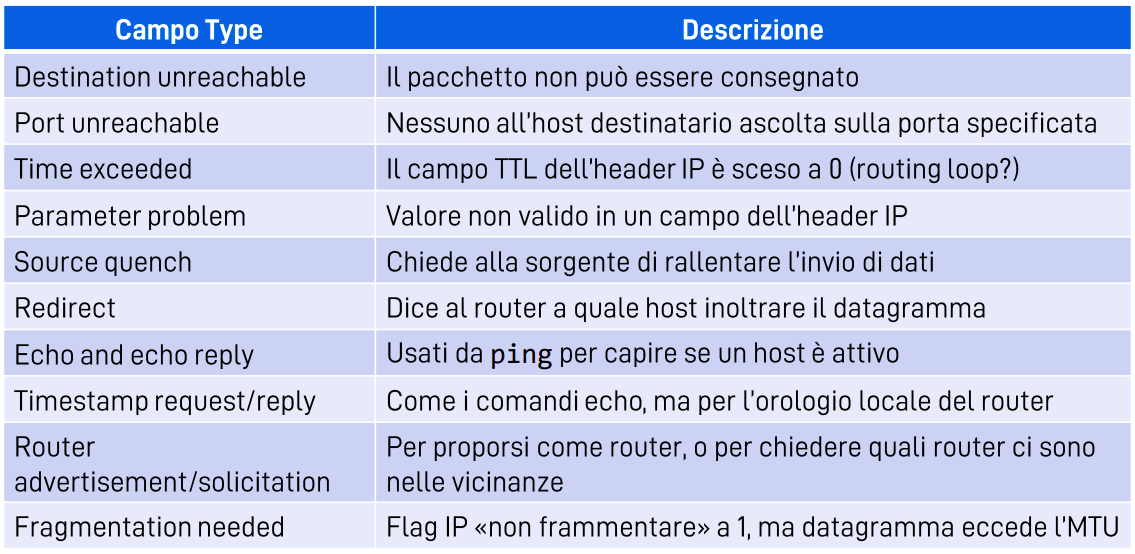
\includegraphics[width=0.85\textwidth]{messaggio-icmp.png}
    \caption{Tipi di messaggi \emph{ICMP}}
\end{figure}

I messaggi possono essere distinti in due classi: quelli per la segnalazione
di errori (e.g. \texttt{Time Exceeded} e \texttt{Destination Unreachable}) e
quelli usati per recuperare informazioni (e.g. \texttt{Echo Request e Echo Reply}).

\begin{note}
    Per evitare di congestionare la rete, \emph{ICMP} è progettato per non
    segnalare errori provocati da altri messaggi \emph{ICMP}.
\end{note}

\subsection{Ping tramite ICMP}
Il comando \texttt{ping} è implementato sfruttando le \texttt{Echo Request} e le
\texttt{Echo Reply}. Con una \texttt{Echo Request} viene trasmesso un messaggio e
il destinatario esegue una \texttt{Echo Reply} ritrasmettendo indietro lo stesso
messaggio ricevuto.

Questo comportamento permette di verificare la raggiungibilità di un \emph{host}
e di misurarne l'\emph{\gls{glos:RTT}}.

\subsection{Traceroute tramite ICMP}
Vengono inviati pacchetti \emph{IP} con \emph{\gls{glos:TTL}} sempre maggiore
(1, 2, 3, \dots) fino a quando non viene raggiunta la destinazione. Ogni volta
che un \emph{router} scarta un \emph{pacchetto} con \emph{TTL} nullo, trasmette un
messaggio \emph{ICMP} di tipo \texttt{Time Exceeded} con il proprio \emph{IP}.

L'insieme di tutti i messaggi \emph{ICMP} ricevuti permette di tracciare la rotta
seguita dal un \emph{pacchetto} per raggiungere una certa destinazione.

\section{Protocollo DHCP}
\subsection{Principio di funzionamento}
Il \emph{\gls{prot:DHCP}} è un protocollo client-server che permette di assegnare
dinamicamente gli \emph{indirizzi IP} agli \emph{host} di una rete. La procedura
di assegnamento, in sintesi, si compone di 4 fasi:
\begin{enumerate}
    \item L'\emph{host} invia un messaggio \texttt{DHCP discover};
    \item Il server \emph{DHCP} risponde inviano con un messaggio \texttt{DHCP
    offer};
    \item L'\emph{host} accetta l'offerta del server;
    \item Il server risponde con un \emph{DHCP ACK};
\end{enumerate}
Poiché il client non ha un \emph{indirizzo IP} tutte le comunicazioni avvengono
in \emph{broadcast}, ovvero il client contatta il server indicando come
indirizzo sorgente $0.0.0.0$, mentre il server risponde all'indirizzo $255.255.255.255$.

\noindent
Per distinguere tra loro più transazioni viene usato un \texttt{transaction ID}
generato casualmente dal client. Il server risponde ad ogni richiesta indicando
nei messaggi lo stesso valore di \texttt{transaction ID} della richiesta. In
questo modo i client possono capire se la risposta è o meno destinata a loro.

\begin{figure}[ht]
    \centering
    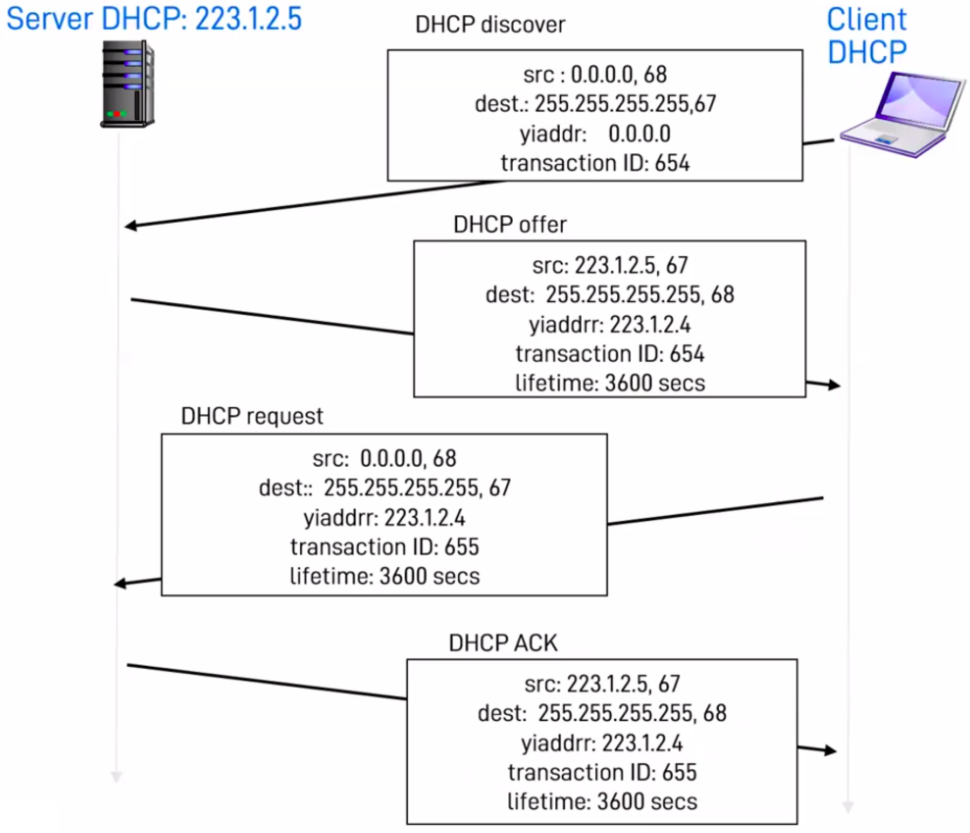
\includegraphics[width=0.8\textwidth]{transazioni-dhcp.png}
    \caption{Transazioni \emph{DHCP}}
\end{figure}\noindent
Il campo \texttt{yiaddr} (your ip address) contiene l'\emph{indirizzo IP} che il
server \emph{DHCP} propone al client.

\begin{note}
    Il protocollo \emph{DHCP} è un protocollo del \emph{livello Applicativo},
    infatti, server e client sono identificati da una \emph{socket}. In
    particolare, il server opera sulla porta 67, mentre il client sulla 68.
    Inoltre, il \emph{DHCP} utilizza il protocollo \emph{UDP} e non potrebbe
    fare altrimenti visto che il client non ha un \emph{indirizzo IP} con il
    quale instaurare una connessione \emph{TCP}. Ovviamente, la gestione di
    perdite e duplicazioni è gestita bene dal protocollo.
\end{note}

\subsection{Gestione dei prestiti}
L'\emph{indirizzo IP} fornito dal \emph{DHCP} è valido per una certa quantità di
tempo al termine del quale, l'indirizzo ritorna disponibile per altre assegnazioni.
Al termine di un prestito il client può richiedere un nuovo \emph{IP} o
l'estensione del prestito.

Solitamente i client, prima dello scadere del tempo, chiedono il rinnovo al server
e questo generalmente lo autorizza. Il motivo per il quale il server tende ad
autorizzare i rinnovi è che altrimenti gli \emph{host} dovrebbero richiedere un
nuovo indirizzo e riaprire tutte le connessioni che stavano utilizzando, causando
molto traffico all'interno della rete. Tuttavia, qualora il server neghi
l'estensione di un prestito, il client deve obbligatoriamente smettere di usare
quell'indirizzo per non causare collisioni.

\begin{note}
    Oltre all'\emph{indirizzo IP}, il \emph{DHCP} fornisce anche altre informazioni
    quali il \emph{default gateway}, la \emph{netmask} (o \emph{subnetmask}) e
    il nome e l'indirizzo del server \emph{\gls{prot:DNS}}.
\end{note}

\subsection{Messaggi DHCP}
\begin{figure}[h!]
    \centering
    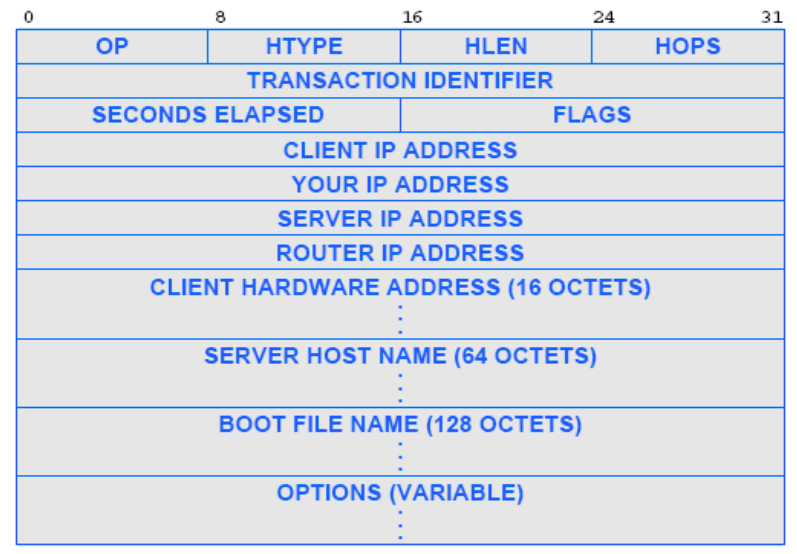
\includegraphics[width=0.8\textwidth]{messaggio-dhcp.png}
    \caption{Struttura di un messaggio \emph{DHCP}}
\end{figure}\noindent
Vediamo nel dettaglio il significato dei vari campi:
\begin{itemize}
    \item \texttt{OP}: specifica se si tratta di una richiesta o di una risposta;
    \item \texttt{HTYPE}: specifica il tipo di interfaccia hardware utilizzata;
    \item \texttt{HLEN}: specifica la lunghezza dell'\emph{indirizzo MAC};
    \item \texttt{FLAGS}: specifica se il mittente può ricevere broadcast o
    risposte dirette;
    \item \texttt{HOPS}: specifica quanti server hanno inoltrato la richiesta;
    \item \texttt{TRANSACTION IDENTIFIER}: è usato per far corrispondere le
    risposte alle richieste;
    \item \texttt{SECOND ELAPSED}: indica i secondi passati da quando l'\emph{host}
    è entrato in funzione;
    \item \texttt{CLIENT IP ADDRESS}: \emph{indirizzo IP} del client \emph{DHCP};
    \item \texttt{YOUR IP ADDRESS}: \emph{indirizzo IP} proposto dal server
    (inizialmente vale $0.0.0.0$);
    \item \texttt{SERVER IP ADDRESS}: \emph{indirizzo IP} del server \emph{DHCP};
    \item \texttt{SERVER HOST NAME}: \emph{nome di dominio} del server \emph{DHCP};
    \item \texttt{ROUTER IP ADDRESS}: indirizzo del \emph{default gateway};
    \item \texttt{CLIENT HARDWARE ADDRESS}: \emph{indirizzo MAC} del client \emph{DHCP};
    \item \texttt{BOOT FILE NAME}: percorso di un file con istruzioni per configurare
    un il client all'avvio;
\end{itemize}
\begin{note}
    Tutti i campi, ad eccezione di \texttt{OPTIONS}, hanno una dimensione fissa.
\end{note}

\subsection{Reti senza DHCP}
Se una rete non ha un server \emph{DHCP} e gli \emph{host} non sono stati configurati
staticamente\footnotemark, ogni \emph{host} si autoassegna un \emph{indirizzo
link-local}. Ovviamente, per assicurarsi che l'indirizzo scelto non sia già stato
preso, ogni \emph{host} trasmette una richiesta \emph{ARP} contenente l'\emph{IP}
che si è assegnato. Se nessuno risponde si tiene l'indirizzo, altrimenti ne sceglie
un altro e ripete l'operazione.

In realtà, è possibile configurare i \emph{router} in modo che, per i soli
messaggi \emph{DHCP}, non blocchino i \emph{pacchetti} con indirizzo
$255.255.255.255$ consentendo in questo modo l'utilizzo di server \emph{DHCP}
risiedenti su reti diverse.

\footnotetext{Negli \emph{host} configurati staticamente l'amministratore di rete
inserisce tutte le informazioni necessarie}

\section{Il viaggio di un pacchetto attraverso la rete}
Vediamo ora come viene trattato complessivamente un \emph{pacchetto} dal momento
dell'invio fino alla sua ricezione.

Prendiamo la seguente rete:

\begin{figure}[h!]
    \centering
    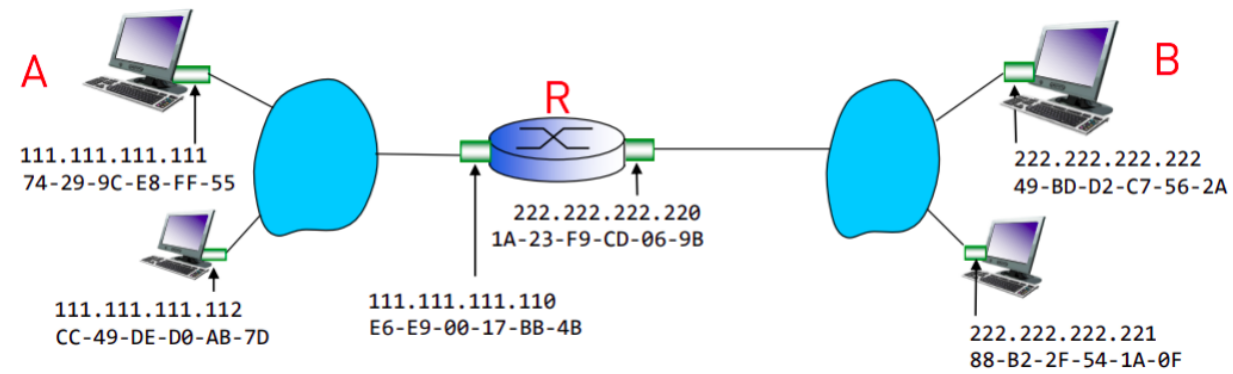
\includegraphics[width=\textwidth]{rete-ip-esempio.png}
    \caption{Esempio di \emph{rete IP}}
\end{figure}\noindent
Supponiamo che l'\emph{host} $A$ voglia inviare un \emph{pacchetto} all'\emph{host}
$B$ e che $A$ conosca già l'\emph{indirizzo IP} di $B$ e gli \emph{indirizzi IP}
e \emph{MAC} del \emph{router}\footnotemark.

\footnotetext{$A$ può conoscere l'\emph{IP} del \emph{router} grazie al
\emph{DHCP} e il \emph{MAC} grazie all'\emph{ARP}}

Quindi, $A$ crea un \emph{pacchetto}, impostando come sorgente il proprio \emph{IP}
e come destinazione l'\emph{indirizzo IP} di $B$, e lo incapsula in un
\emph{frame} nel quale gli indirizzi di sorgente e di destinazione sono
rispettivamente il proprio \emph{MAC} e il \emph{MAC} di $R$.

$R$ riceve il \emph{frame}, ne estrae il \emph{pacchetto} e analizzando la
propria tabella di inoltro decide verso quale interfaccia inviarlo. In questo
caso, sceglie l'interfaccia con indirizzo $222.222.222.220$ e con
\emph{next hop} \quotes{\texttt{diretto}}.

A questo punto, se $R$ conosce l'\emph{indirizzo MAC} di $B$ crea un \emph{frame}
indicandolo come indirizzo di destinazione, altrimenti invia un messaggio
\emph{ARP} in broadcast sulla rete di $B$, $B$ risponde indicando il proprio
\emph{MAC} e $R$ lo salva nella propria \emph{cache ARP}.

Infine, $B$ riceve il \emph{frame} e ne estrae il \emph{pacchetto}.

\section{Protocollo IPv6}
Il protocollo \emph{IPv6} è un'evoluzione dell'\emph{IP}, o meglio dell'\emph{IPv4},
ed è nato per ampliare la quantità di indirizzi disponibili, velocizzare
l'elaborazione dei \emph{pacchetti} introducendo header di dimensione fissa e
migliorare la gestione della \quotes{qualità del servizio}.

\subsection{Struttura dei pacchetti IPv6}
I \emph{pacchetti IPv6} hanno uno o più header di dimensione fissa $40byte$
e sono organizzati come da figura sottostante:
\begin{figure}[h!]
    \centering
    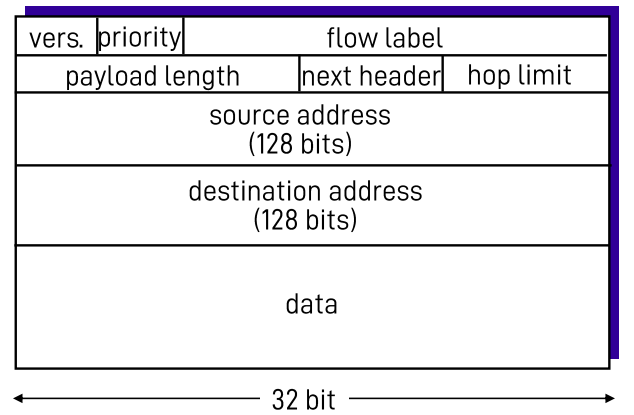
\includegraphics[width=0.6\textwidth]{messaggio-ipv6.png}
    \caption{Struttura di un \emph{pacchetto IPv6}}
\end{figure}
I campi sono molti meno rispetto all'\emph{IPv4} e ce ne sono di nuovi:
\begin{itemize}
    \item \texttt{Version}: indica la versione del protocollo;
    \item \texttt{Priority}: indica la priorità dei \emph{pacchetti} che fanno
    parte dello stesso \emph{flusso};
    \item \texttt{Flow label}: etichetta che identifica il \emph{flusso}
    di appartenenza dei \emph{pacchetti};
    \item \texttt{Payload length}: dimensione del payload;
    \item \texttt{Next header}: identifica il protocollo di livello 4 incapsulato
    nei dati;
    \item \texttt{Hop limit}: numero di \emph{hop} rimasti al \emph{pacchetto};
    \item \texttt{Source address}: indirizzo sorgente;
    \item \texttt{Destination address}: indirizzo di destinazione;
    \item \texttt{Data}: payload del \emph{pacchetto} o header successivo;
\end{itemize}
I campi \texttt{Checksum} e \texttt{Options} sono stati rimossi, ma come già
detto, è possibile inserire un secondo header impostando un valore adeguato nel
campo \texttt{Next header}.

\begin{note}
    È stato modificato anche il protocollo \emph{ICMP}, introducendo l'\emph{ICMPv6}
    che aggiunge nuovi messaggi di errore, quale ad esempio il \texttt{Packet too
    big}, e funzioni per la gestione dei gruppi \emph{multicast}.
\end{note}

\subsection{Tunneling tramite IPv4}
Poiché molti \emph{router} ancora non supportano l'\emph{IPV6}, per permettere a
\emph{IPv4} e \emph{IPv6} di coesistere, è stata introdotto il concetto di
\emph{tunneling}, ovvero, è possibile far viaggiare \emph{pacchetti IPv6}
attraverso porzioni di rete che non supportano \emph{IPv6}, incapsulandoli
all'interno di \emph{pacchetti IPv4}.

\begin{figure}[ht]
    \centering
    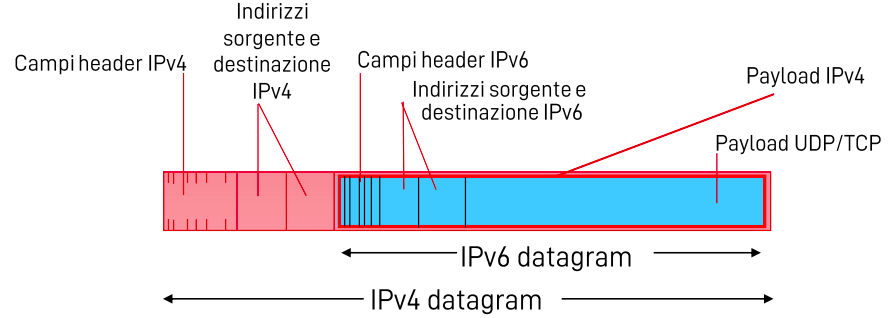
\includegraphics[width=\textwidth]{tunneling-ipv6.png}
    \caption{\emph{Tunneling IPv6}}
\end{figure}
\begin{figure}[ht!]
    \centering
    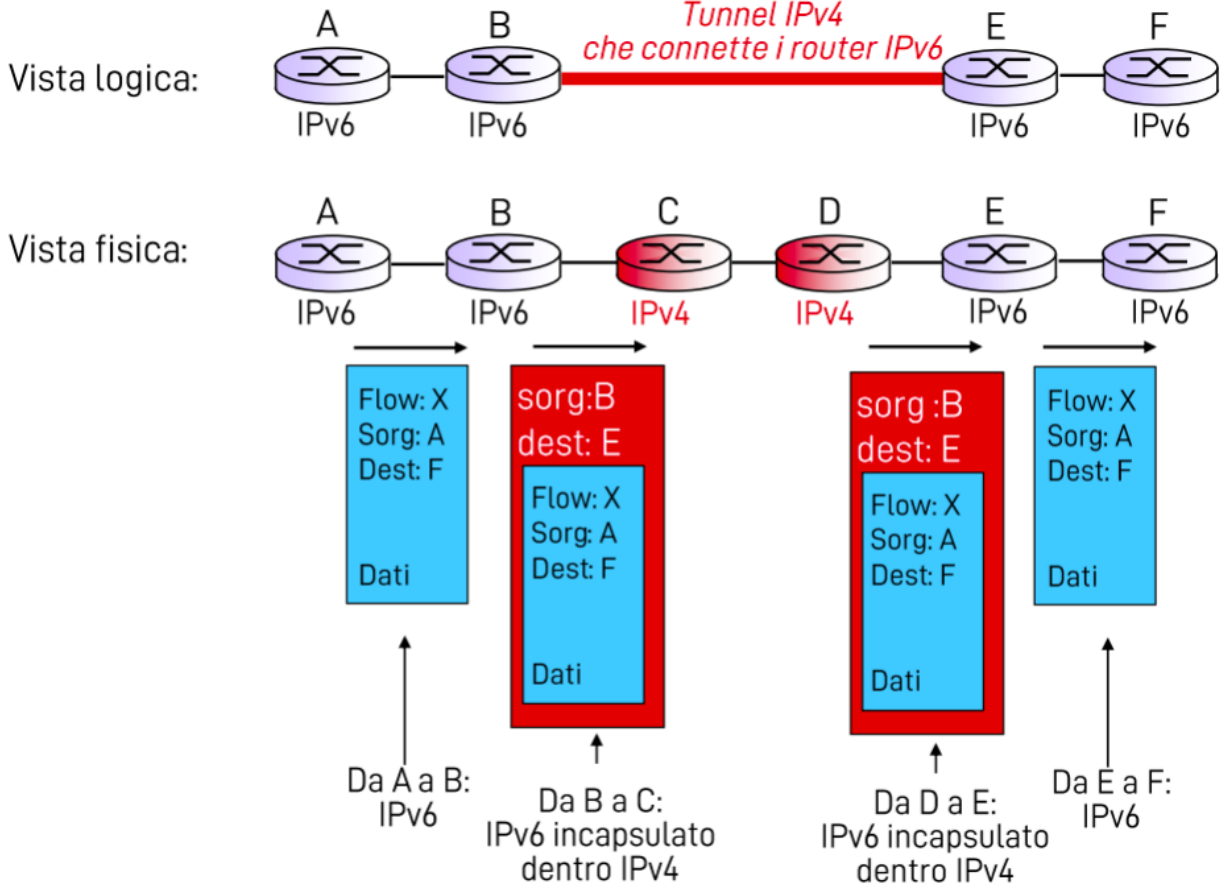
\includegraphics[width=\textwidth]{tunneling-ipv6-vista.png}
    \caption{\emph{Tunneling IPv6} vista logica e fisica}
\end{figure}

\newpage
\subsection{Struttura e tipologia di indirizzi IPv6}
Gli \emph{indirizzi IPv6} sono codificati su 128 bit e a differenze di
\emph{IPv4}, vengono rappresentati da 32 cifre esadecimali divise in 8 gruppi
da 4, ad esempio:
\[\texttt{2a03:2880:f108:0083:face:b00c:0000:25de}\]
Per accorciarli è possibile omettere gli zeri iniziali di un quartetto e indicare
con un solo zero un quartetto formato da quattro zeri, ad esempio l'indirizzo di
prima può essere espresso come:
\[\texttt{2a03:2880:f108:83:face:b00c:0:25de}\]
Qualora vi siano più quartetti consecutivi di zeri, è possibile ometterli
indicando al loro posto $::$. Ad esempio il seguente indirizzo:
\[\texttt{2a03:2880:f108:0000:0000:0000:0000:25de}\]
diventa:
\[\texttt{2a03:2880:f108::25de}\]
Tuttavia, se esistono più gruppi di zeri, si può omettere solo il gruppo
più lungo, altrimenti non si sarebbe più in grado di stabilire la forma completa
dell'indirizzo.

\paragraph{CIDR IPv6}
In \emph{IPv6} prefissi e suffissi sono gestiti col metodo \emph{\gls{glos:CIDR}}
come in \emph{IPv4}, ad esempio la seguente rete:
\[\texttt{2a03:2880:f108:83::/64}\]
comprende gli indirizzi da:
\[\texttt{2a03:2880:f108:83:0:0:0:0}\]
a:
\[\texttt{2a03:2880:f108:83:ffff:ffff:ffff:ffff}\]

\bigskip\noindent
Solitamente il prefisso è a sua volta diviso in \emph{prefisso di routing}
che identifica un'azienda o un'organizzazione e un \emph{SubnetID} che
identifica una specifica sottorete di quella organizzazione.
\begin{figure}[ht!]
    \centering
    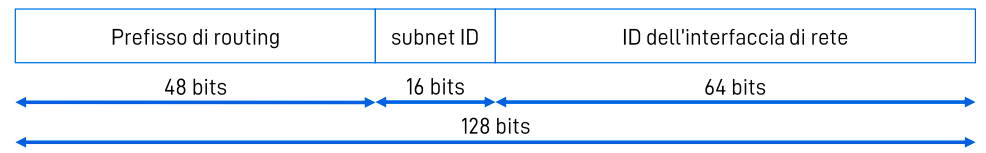
\includegraphics[width=\textwidth]{cidr-ipv4.png}
    \caption{Tipica suddivisione di un \emph{indirizzo IPv6}}
\end{figure}

\paragraph{Indirizzi speciali}
Anche in \emph{IPv6} esistono gli stessi indirizzi speciali visti nell'\emph{IPv4},
ma la definizione di alcuni è diversa:
\begin{itemize}
    \item \emph{Indirizzo \quotes{questo computer}}: è una stringa di 128 zeri
    che in notazione semplificata sono rappresentabili come $\texttt{::/128}$;
    \item \emph{Indirizzo loopback}: ce n'è solo uno ed è $\texttt{::1/128}$;
    \item \emph{Indirizzi multicast}: sono tutti gli indirizzi della sottorete
    $\texttt{ff08::/8}$;
    \item \emph{Link-local unicast}: corrispondono agli indirizzi \emph{link-local}
    dell'\emph{IPv4} e sono tutti quelli della sottorete $\texttt{fe80::/10}$;
\end{itemize}
È possibile mappare ogni \emph{indirizzo IPv4} in un \emph{indirizzo Ipv6}
semplicemente interpretando i 32 bit dell'indirizzo come 8 caratteri esadecimali
e costruendo l'\emph{indirizzo IPv6} come:
\[\texttt{::ffff:wwxx:yyzz}\]
dove $\texttt{ww.xx.yy.zz}$ sono i bit dell'\emph{indirizzo IPv4}.

Ad esempio, l'\emph{indirizzo Ipv4} $193.175.55.16$ in \emph{IPv6} diventa
$\texttt{::ffff:c1af:3710}$.